\documentclass[a4paper,12pt,final]{article}
\usepackage[scaled=0.9]{luximono}
\usepackage[spanish]{babel}
\usepackage[utf8]{inputenc}
\usepackage[T1]{fontenc}
\usepackage{booktabs}
\usepackage{epstopdf}
\usepackage{floatrow}
\usepackage{geometry}
\usepackage{graphicx}
\usepackage{hyperref}
\usepackage{listings}
\usepackage{multicol}
\usepackage{tabularx}
\usepackage{textcomp}
\usepackage{amsmath}
\usepackage{amssymb}
\usepackage{amstext}
\usepackage{caption}
\usepackage{charter}
\usepackage{wrapfig}
\usepackage{amsbsy}
\usepackage{amsthm}
\usepackage{lipsum}
\usepackage{minted}
\usepackage{natbib}
\usepackage{array}
\usepackage{color}
\usepackage{esint}
\usepackage{float}

% Hyperref setup
\hypersetup{
  pdftitle={Procesamiento de datos digitales. Laboratorio 1},
  pdfauthor={Martín Josemaría Vuelta Rojas},
  pdfpagelayout=OneColumn,
  pdfnewwindow=true,
  pdfdisplaydoctitle=true,
  pdfstartview=XYZ,
  plainpages=false,
  unicode=true,
  bookmarksnumbered=true,
  bookmarksopen=true,
  bookmarksopenlevel=3,
  breaklinks=true,
  colorlinks=true,
  linkcolor=blue,
  pdfborder={0 0 0}
}

% Minted settings
\setminted[matlab]{
  autogobble=true,
  linenos=false,
  bgcolor=grey_lighten_4,
  fontfamily=\ttdefault,
  resetmargins=true,
  stripnl=true,
  breaklines=true
  breakautoindent=true,
  breaksymbolleft=\tiny\ensuremath{\hookrightarrow},
  breaksymbolright=\tiny\ensuremath{\hookleftarrow},
  fontsize=\footnotesize
}

\setminted[javascript]{
  autogobble=true,
  linenos=false,
  bgcolor=grey_lighten_4,
  fontfamily=\ttdefault,
  resetmargins=true,
  stripnl=true,
  breaklines=true
  breakautoindent=true,
  breaksymbolleft=\tiny\ensuremath{\hookrightarrow},
  breaksymbolright=\tiny\ensuremath{\hookleftarrow},
  fontsize=\footnotesize
}

\setminted[text]{
  autogobble=true,
  linenos=false,
  bgcolor=grey_lighten_4,
  fontfamily=\ttdefault,
  resetmargins=true,
  stripnl=true,
  breaklines=true
  breakautoindent=true,
  breaksymbolleft=\tiny\ensuremath{\hookrightarrow},
  breaksymbolright=\tiny\ensuremath{\hookleftarrow},
  fontsize=\footnotesize
}

\geometry{
  a4paper,
  total={210mm,297mm},
  left=20mm,
  right=20mm,
  top=20mm,
  bottom=20mm,
}

\floatsetup[listing]{
  capposition=top,
  style=ruled,
}

\captionsetup[listing]{
  labelfont=bf,
  justification=centering
}

\floatsetup[figure]{
  capposition=top,
  style=ruled,
}

\floatsetup[wrapfigure]{
  capposition=top,
  style=plain,
}

\captionsetup[figure]{
  labelfont=bf,
  justification=centering
}

%% LaTeX commands.
\makeatletter
%% -----------------------------------------------------------------------------
\definecolor{grey_lighten_4}{rgb}{0.9804, 0.9804, 0.9804}
%% Caption name for minted environments
% \SetupFloatingEnvironment{listing}{name=Script}
% \SetupFloatingEnvironment{listing}{listname=Lista de scripts}
\renewcommand{\listingscaption}{Script}
\renewcommand{\listoflistingscaption}{Lista de scripts}
%% Redefinition of \maketitle command
\def\@maketitle{%
  \newpage%
  \null%
  \vskip 0em%
  \begin{flushleft}%
      \let \footnote \thanks%
      {\LARGE \@title \par}%
  \end{flushleft}%
  \begin{flushright}%
      \vskip 1em%
      {\@author \par}%
  \end{flushright}%
  \noindent\rule{1\columnwidth}{1pt}%
  \par%
}

\makeatother

%% -----------------------------------------------------------------------------
\begin{document}
  \title{\textit{\Large Laboratorio Nº2}\linebreak{}\linebreak{}\textbf{\Huge Señales}}
  \author{\emph{Martín Josemaría Vuelta Rojas}}
  \maketitle

  \subsection*{Problema 1}
    \noindent Utilizando \textsc{Matlab}, haga un programa (\texttt{function})
    que evalúe las funciones singulares: impulso unitario, escalón unitario
    y función rampa. Debe graficar cada función singular.

    \subsubsection*{Solución}
      \begin{listing}[H]
        \caption{Función impulso unitario}
        \label{script01A}
        \inputminted{matlab}{./laboratorio_2/impulso.m}
      \end{listing}

      \begin{figure}[H]
        \caption{Gráfico de la función impulso unitario del \emph{script \ref{script01A}}.}
        \label{script01Afigure}
        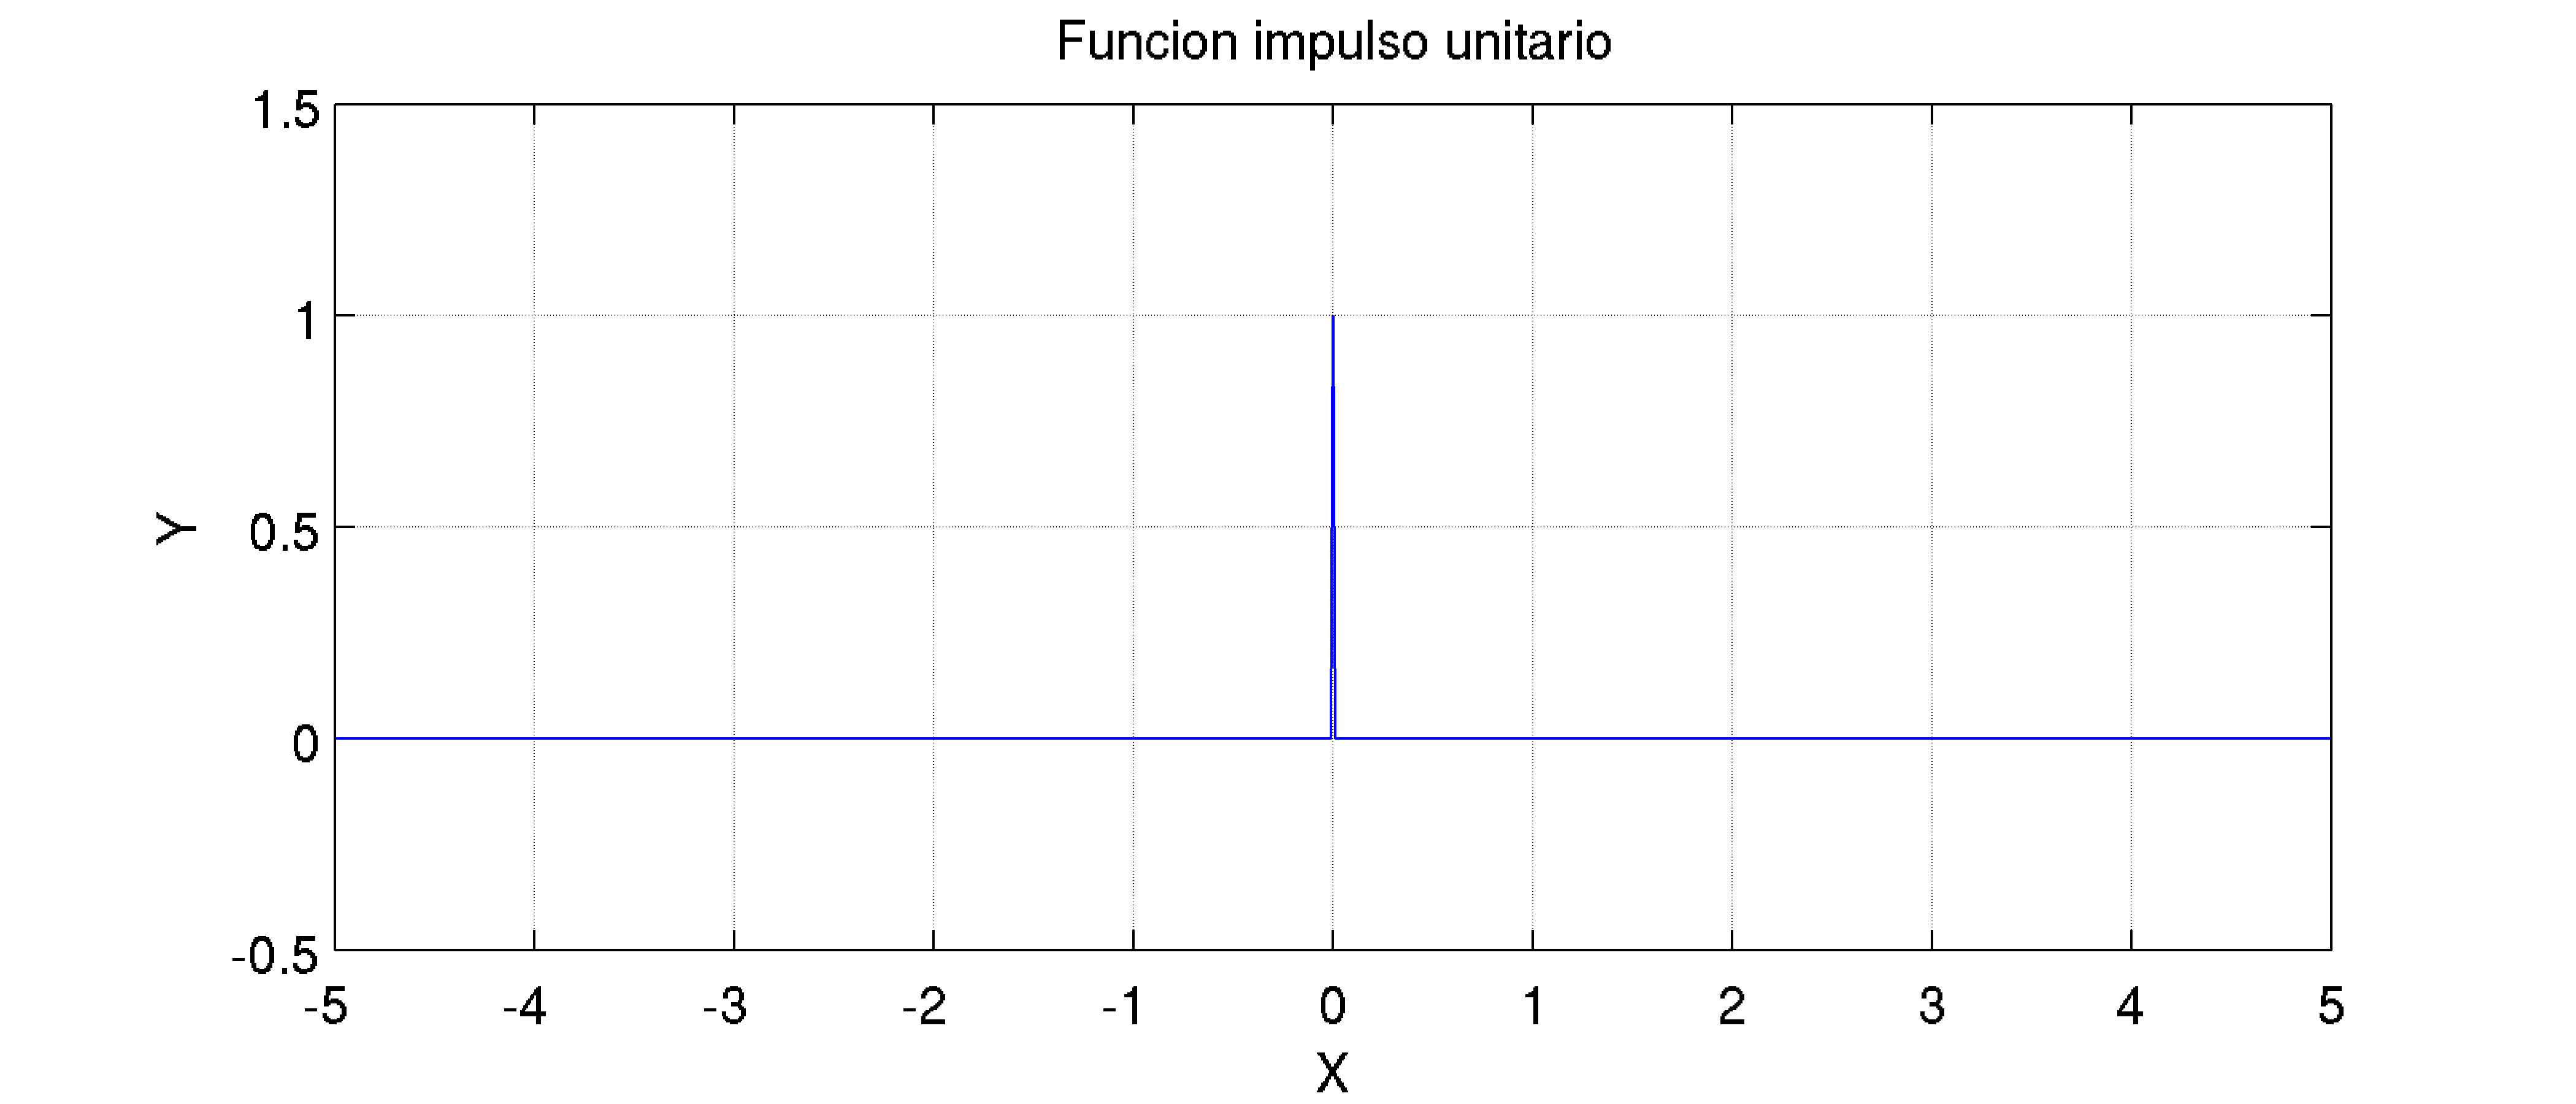
\includegraphics[height=2.5in]{./laboratorio_2/problema01_a.png}
      \end{figure}
      \vspace{\fill}

      \newpage
      \begin{listing}[H]
        \caption{Función escalón unitario}
        \label{script01B}
        \inputminted{matlab}{./laboratorio_2/escalon.m}
      \end{listing}

      \begin{figure}[H]
        \caption{Gráfico de la función escalón unitario del \emph{script \ref{script01B}}.}
        \label{script01Bfigure}
        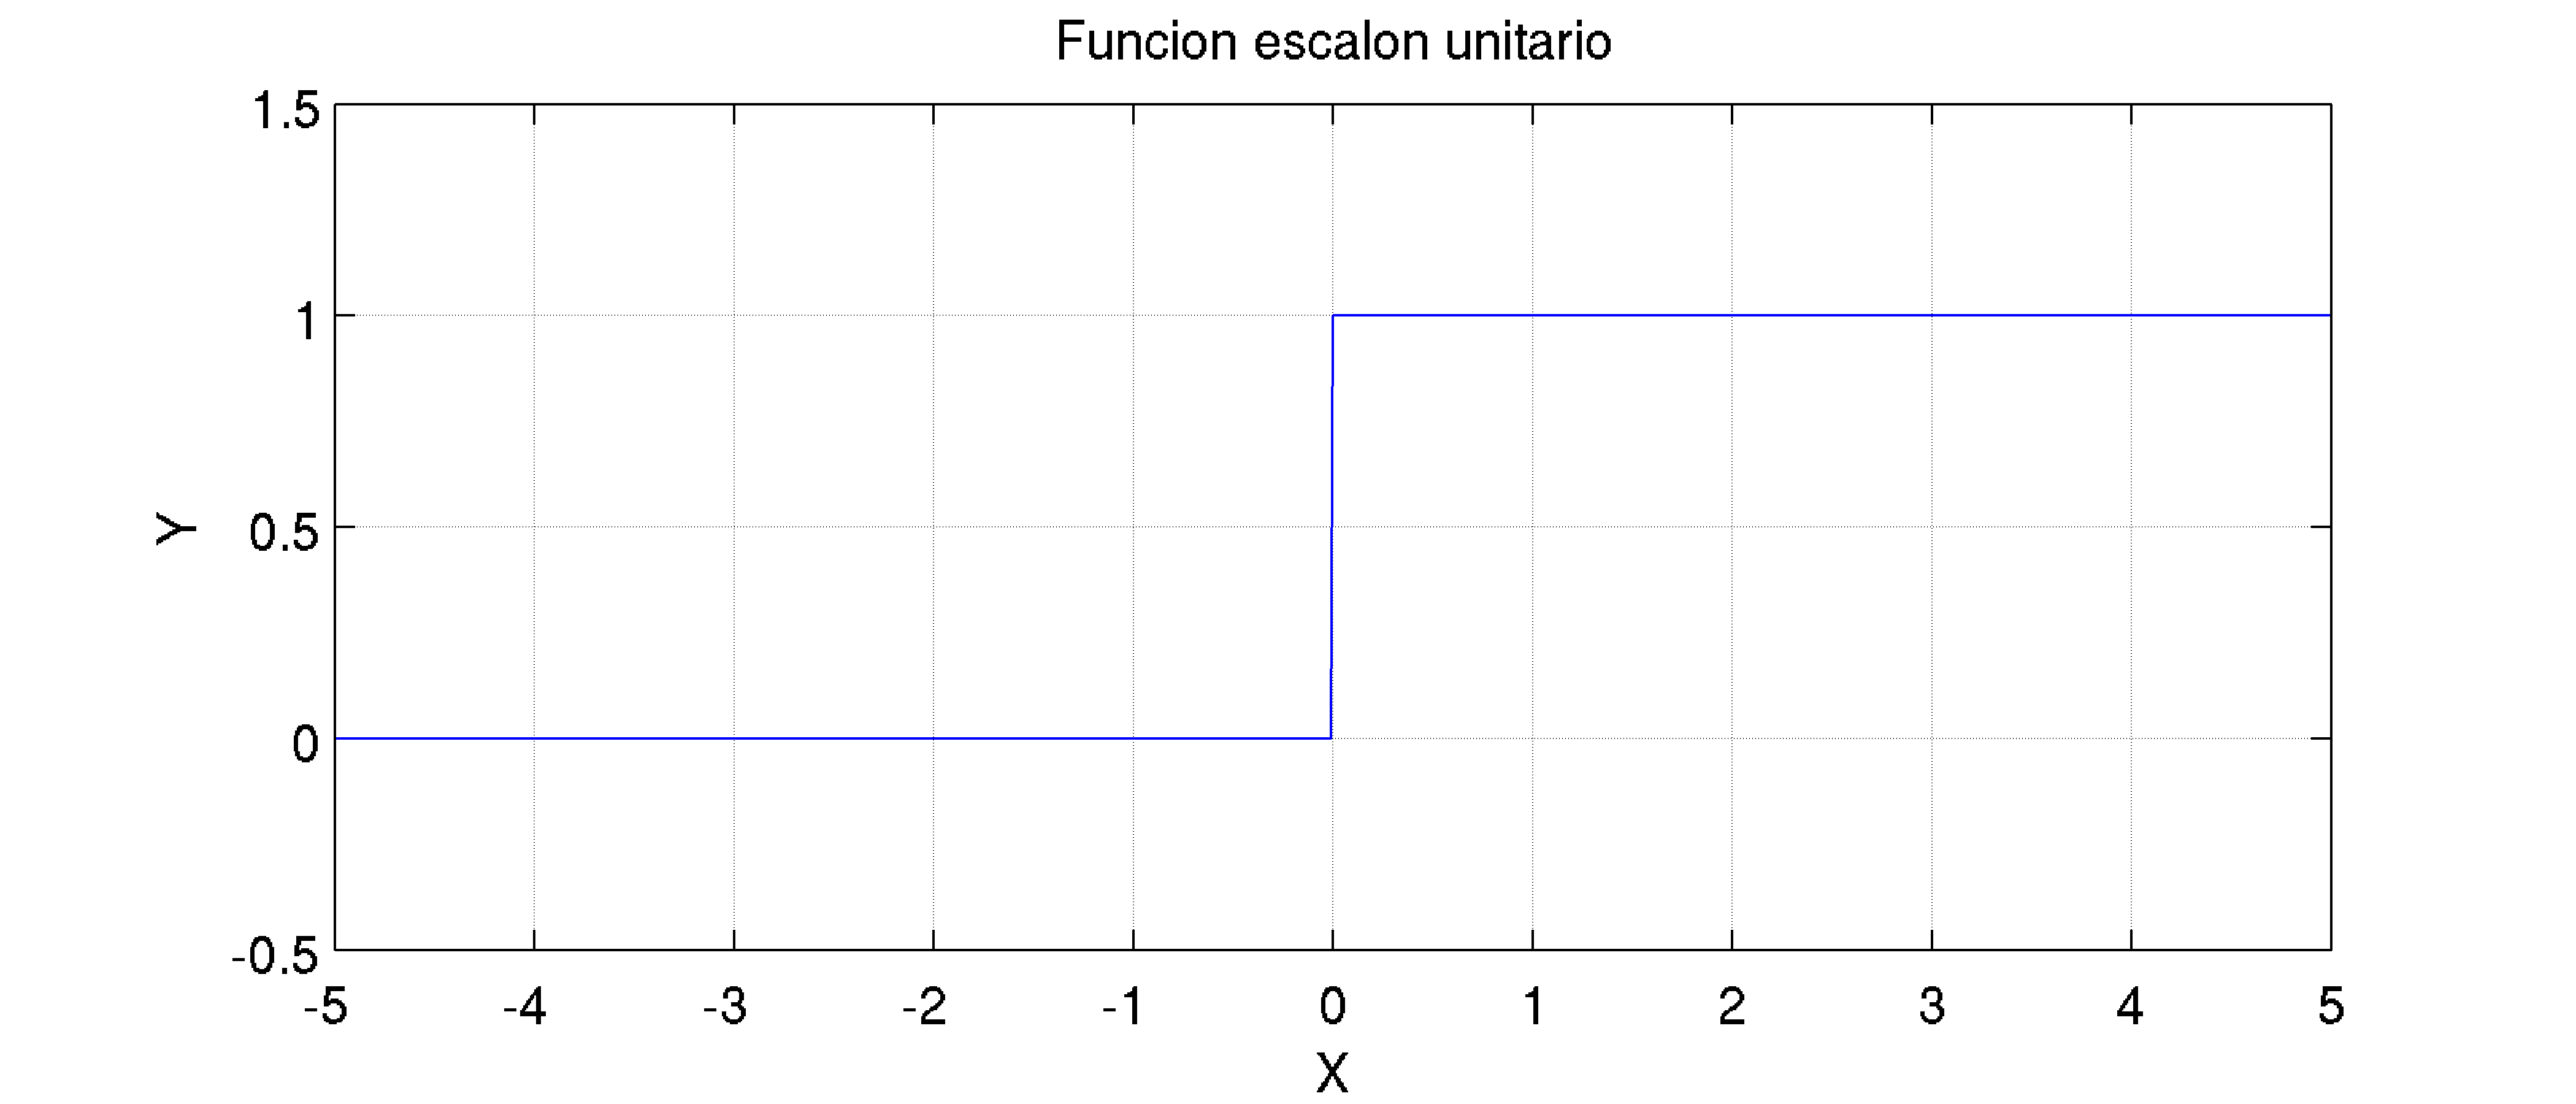
\includegraphics[height=2.5in]{./laboratorio_2/problema01_b.png}
      \end{figure}

      \begin{listing}[H]
        \caption{Función rampa}
        \label{script01C}
        \inputminted{matlab}{./laboratorio_2/rampa.m}
      \end{listing}

      \begin{figure}[H]
        \caption{Gráfico de la función rampa del \emph{script \ref{script01C}}.}
        \label{script01Cfigure}
        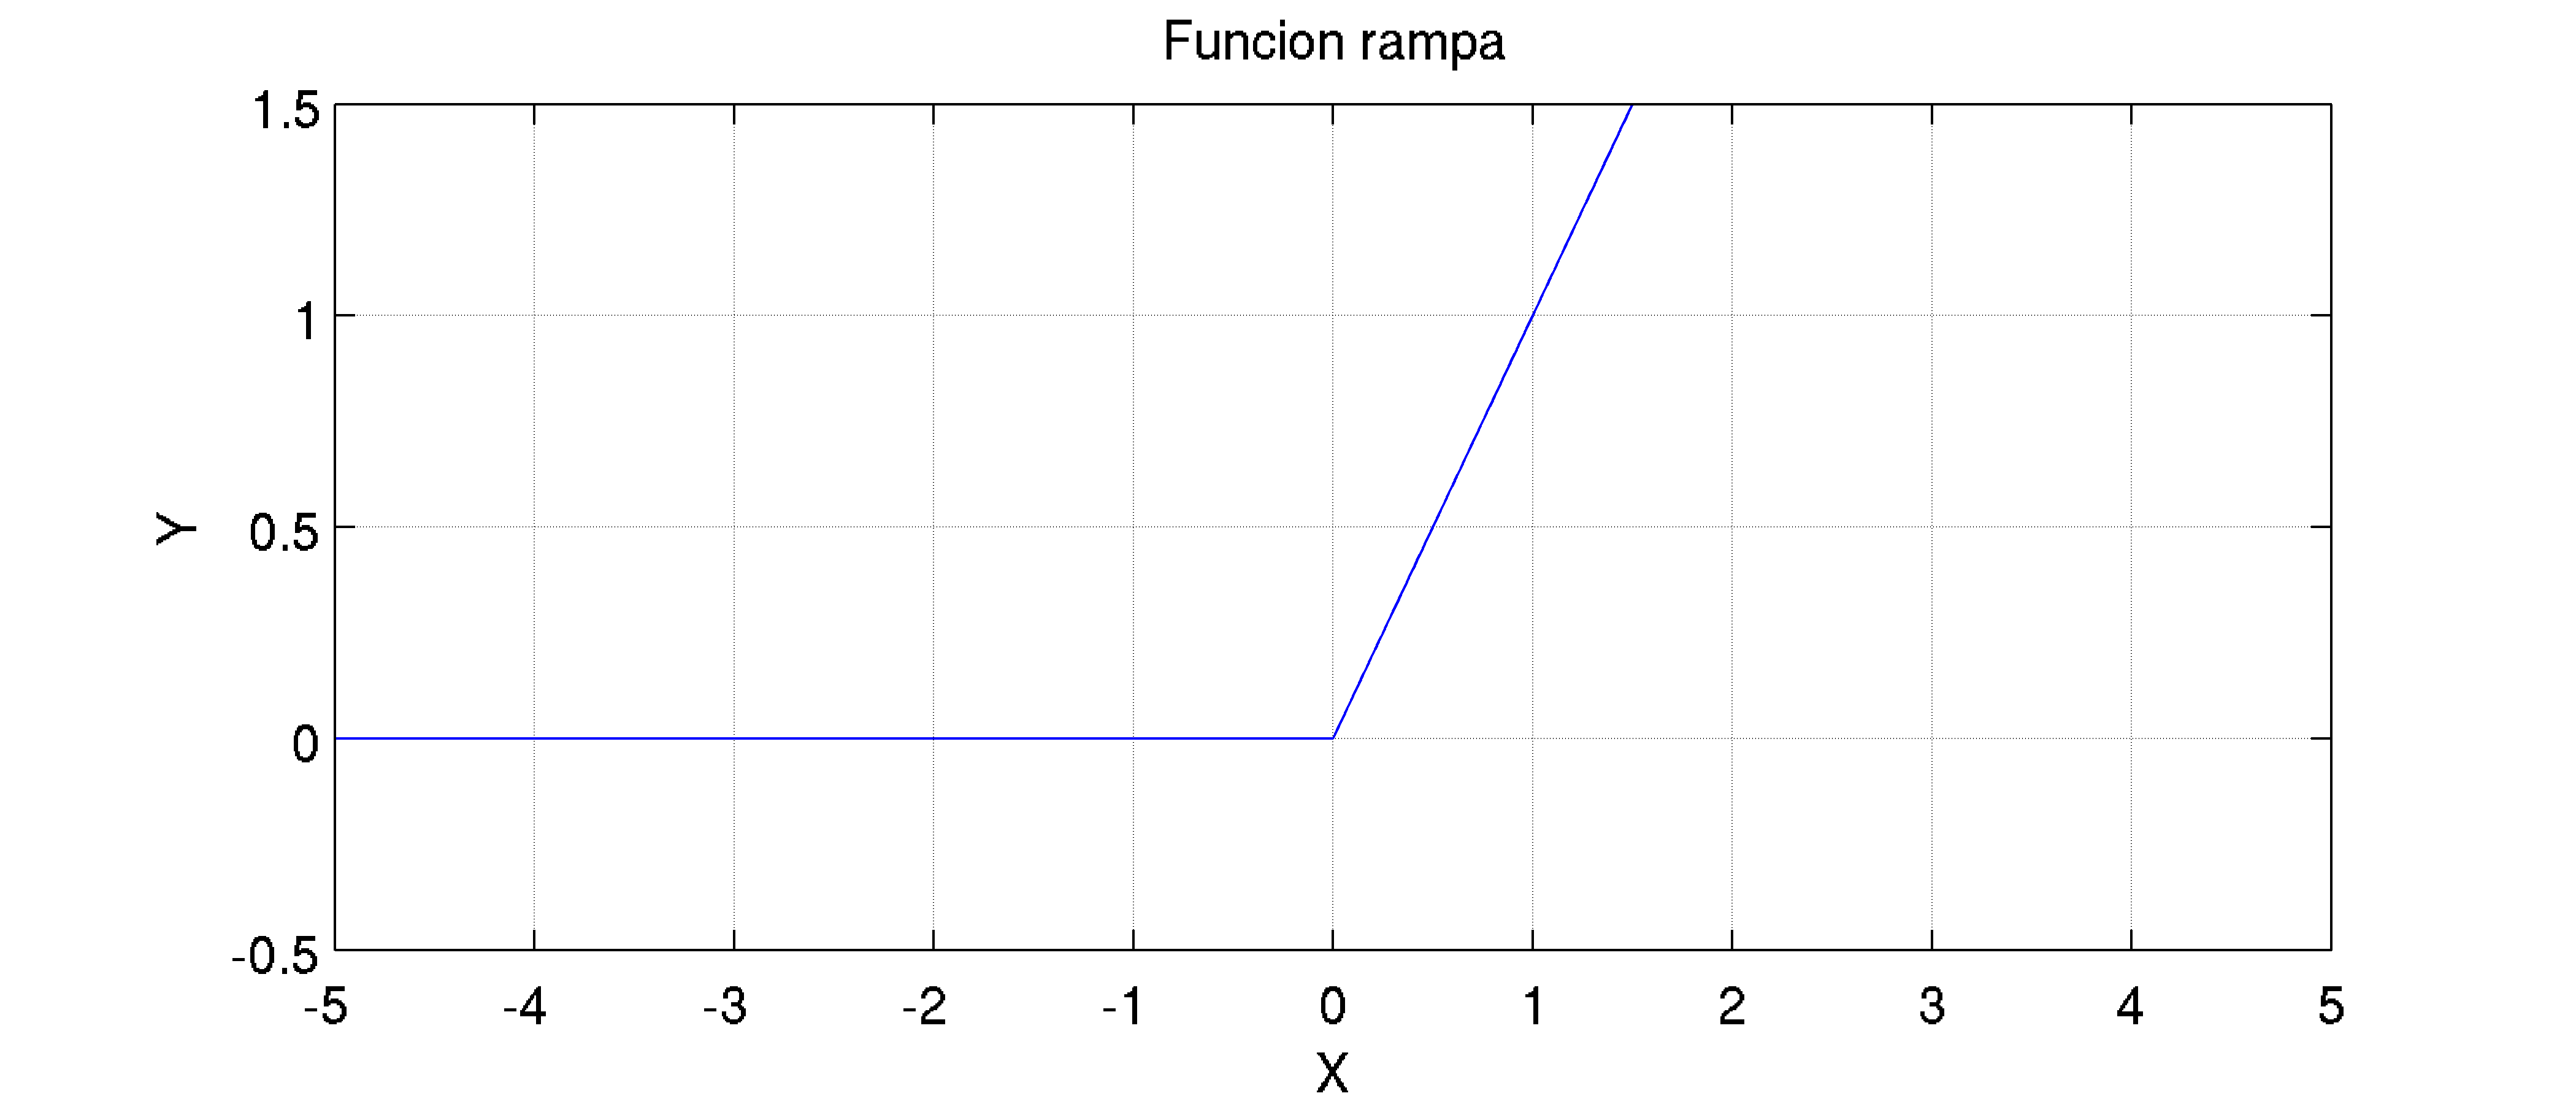
\includegraphics[height=2.5in]{./laboratorio_2/problema01_c.png}
      \end{figure}
      \vspace{\fill}

  \newpage
  \subsection*{Problema 2}
    \noindent Haga un programa para visualizar la función compuerta unitaria de
    \begin{enumerate}
      \item Utilizar los comandos \texttt{zeros} y \texttt{ones}.
      \item Utilizar la función desarrollada en el problema 1.
    \end{enumerate}

    \subsubsection*{Solución}
      \begin{listing}[H]
        \caption{Compuerta unitaria empleando \texttt{zeros} y \texttt{ones}}
        \label{script02A}
        \inputminted[firstline=5]{matlab}{./laboratorio_2/problema02_a.m}
      \end{listing}

      \begin{figure}[H]
        \caption{Resultado de ejecutar el \emph{script \ref{script02A}}.}
        \label{script02Afigure}
        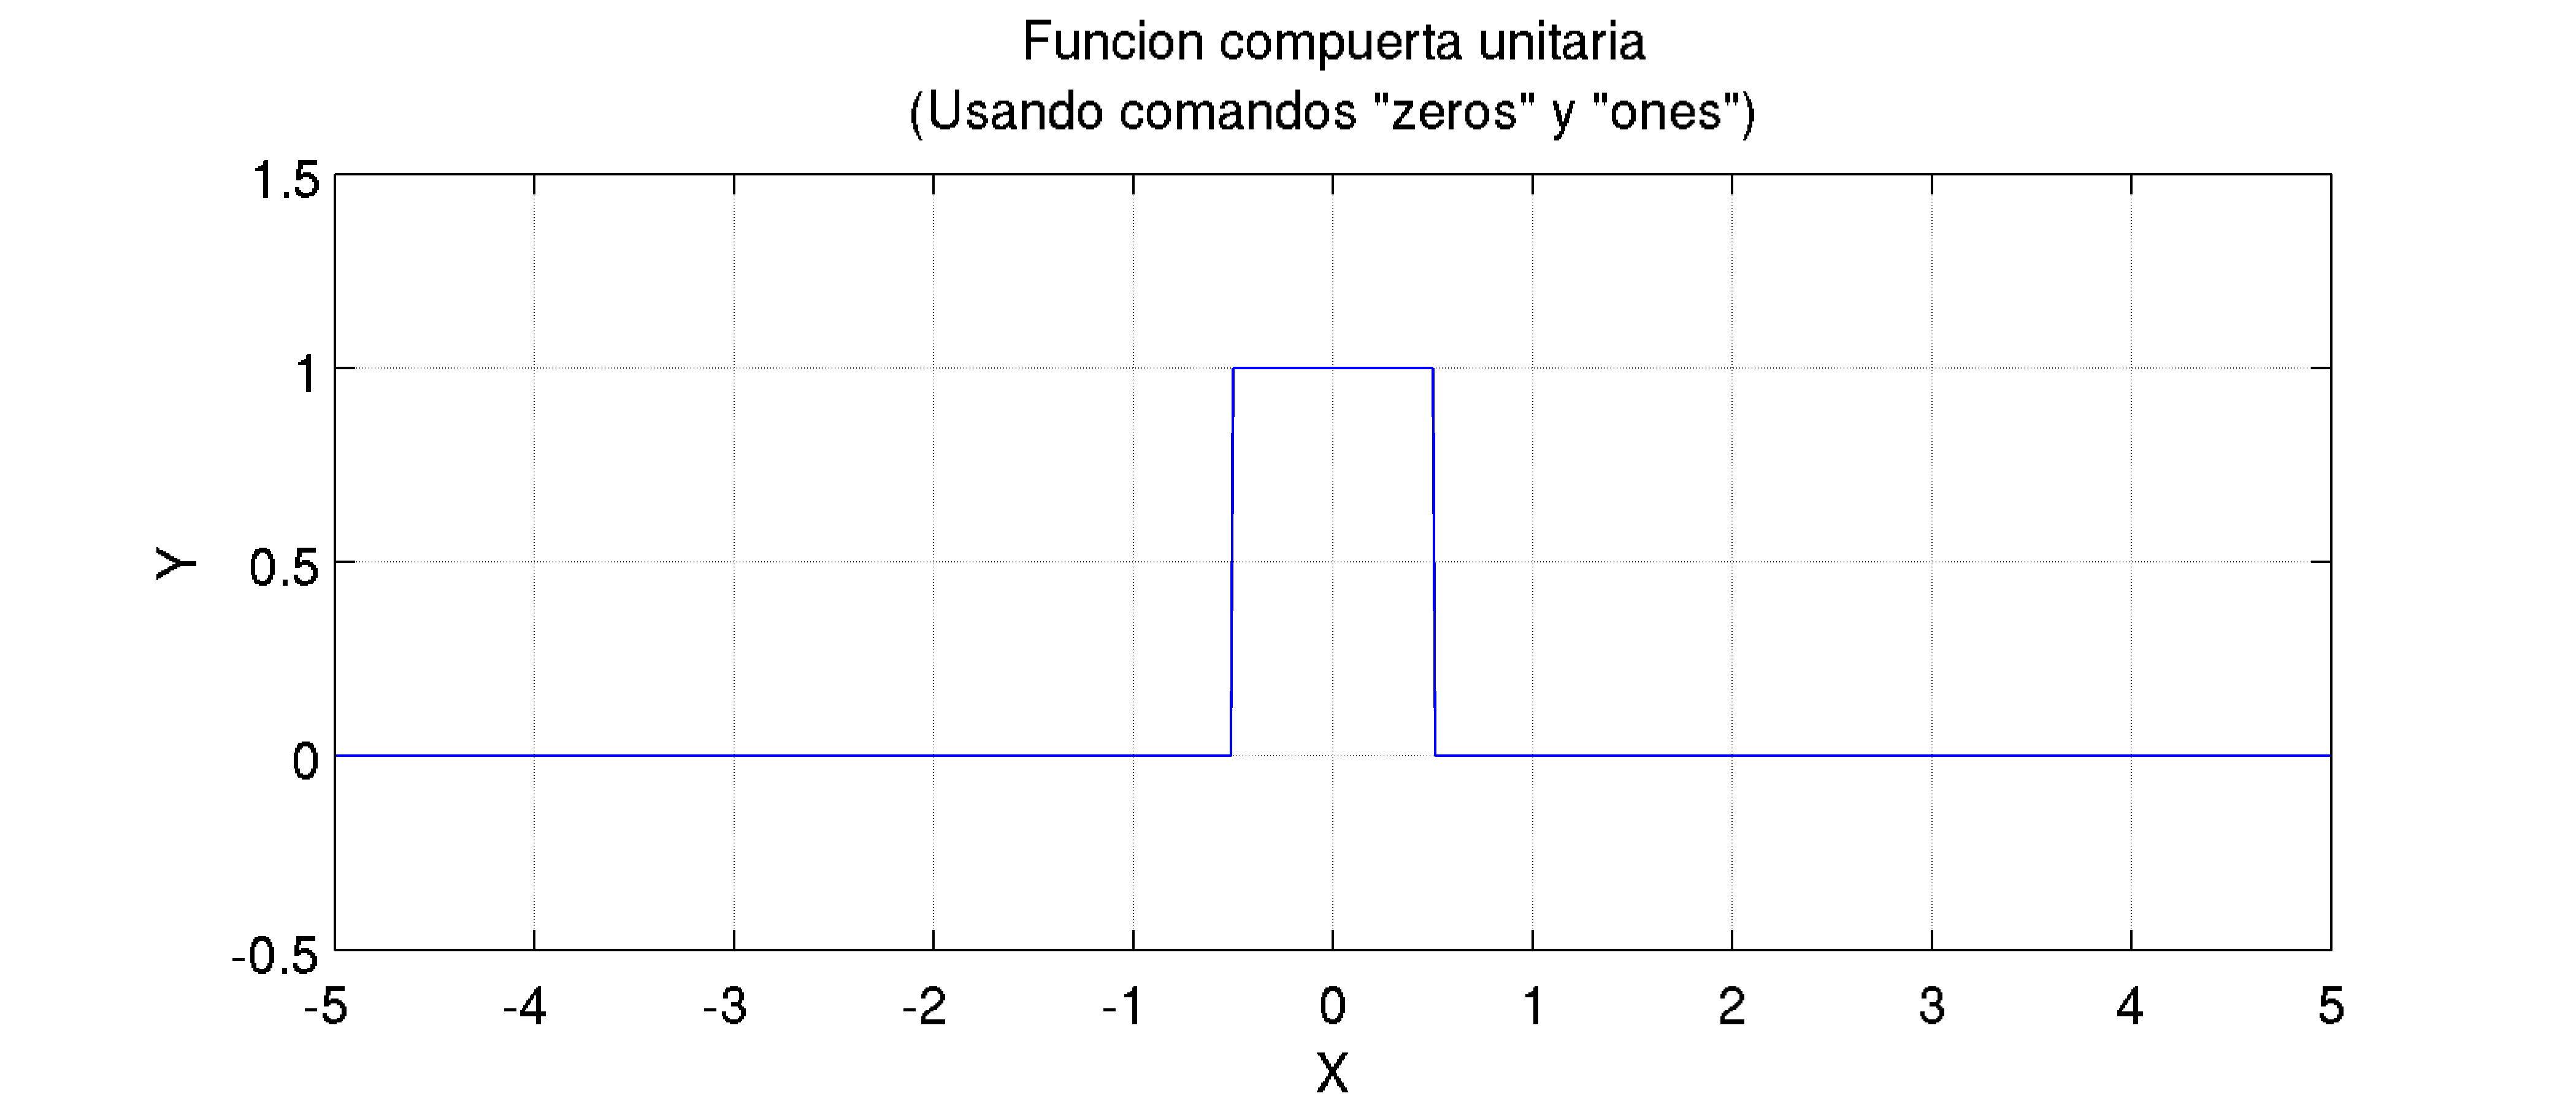
\includegraphics[height=2.5in]{./laboratorio_2/problema02_a.png}
      \end{figure}
      \vspace{\fill}

      \newpage
      \begin{listing}[H]
        \caption{Compuerta unitaria empleando la función \texttt{escalon} desarrollada en el problema 1}
        \label{script02B}
        \inputminted[firstline=5]{matlab}{./laboratorio_2/problema02_b.m}
      \end{listing}

      \begin{figure}[H]
        \caption{Resultado de ejecutar el \emph{script \ref{script02B}}.}
        \label{script02Bfigure}
        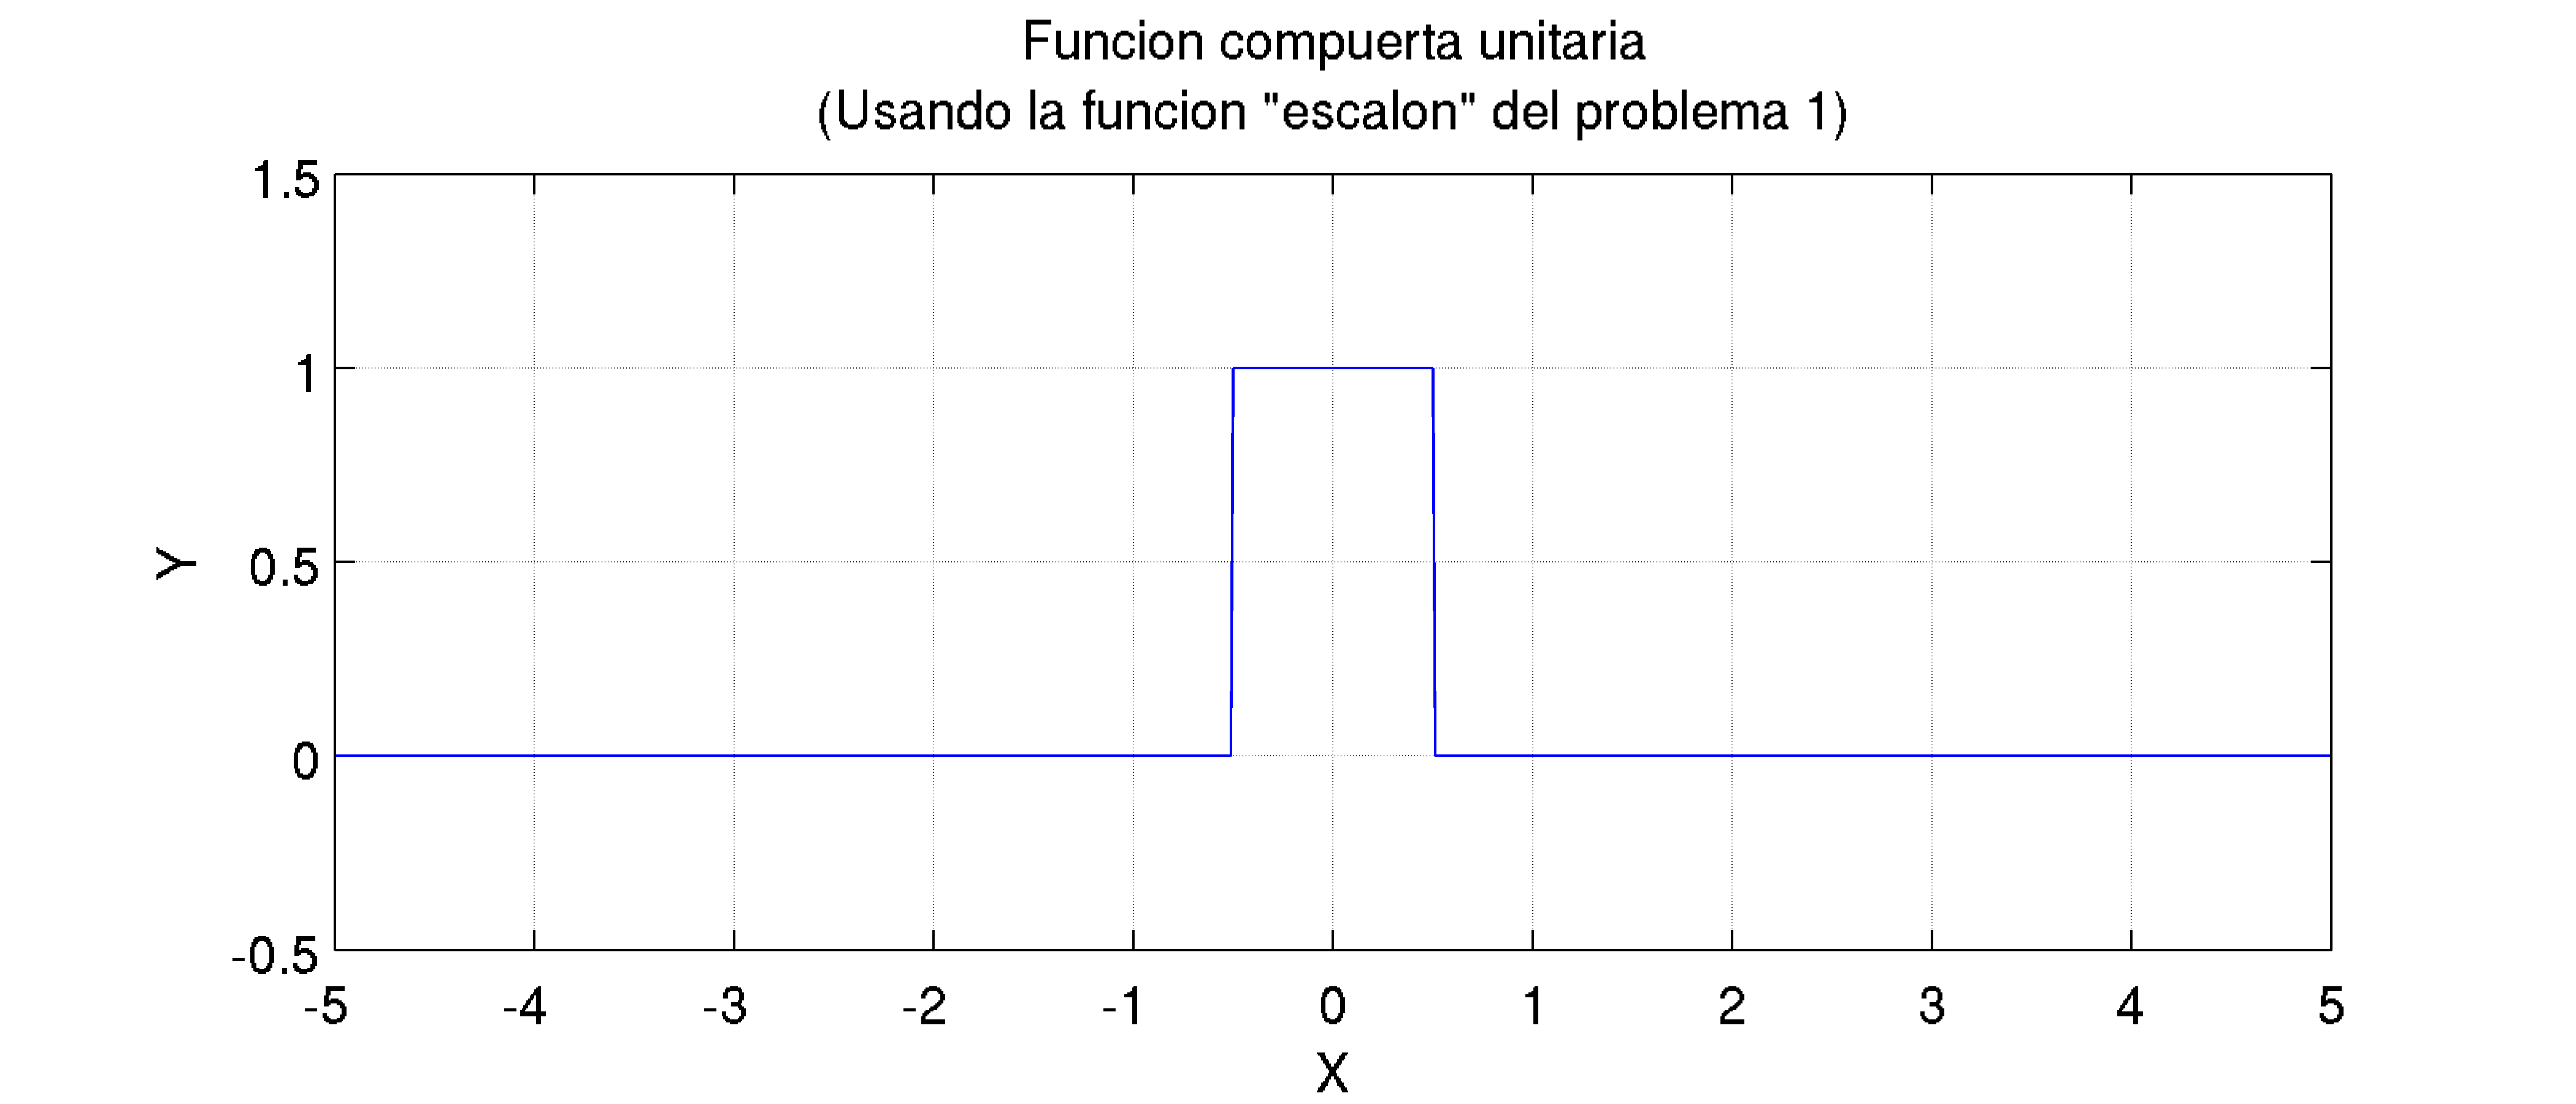
\includegraphics[height=2.5in]{./laboratorio_2/problema02_b.png}
      \end{figure}
      \vspace{\fill}

  \newpage
  \subsection*{Problema 3}
    \noindent Desarrollar un conjunto de comandos \textsc{Matlab} para
    aproximar las siguientes señales periódicas en tiempo continuo, dibujando
    5 ciclos de cada una:
    \begin{enumerate}
        \item Onda Cuadrada, de amplitud 5 Volts, frecuencia fundamental 20 Hz.
        \item Señal diente de sierra, amplitud 5 Volts y frecuencia fundamental 20Hz
    \end{enumerate}

    \subsubsection*{Solución}
      \begin{listing}[H]
        \caption{Función de onda cuadrada}
        \label{script03A}
        \inputminted{matlab}{./laboratorio_2/squarew.m}
      \end{listing}

      \begin{figure}[H]
        \caption{Gráfico de la función rampa del \emph{script \ref{script03A}}.}
        \label{script03Afigure}
        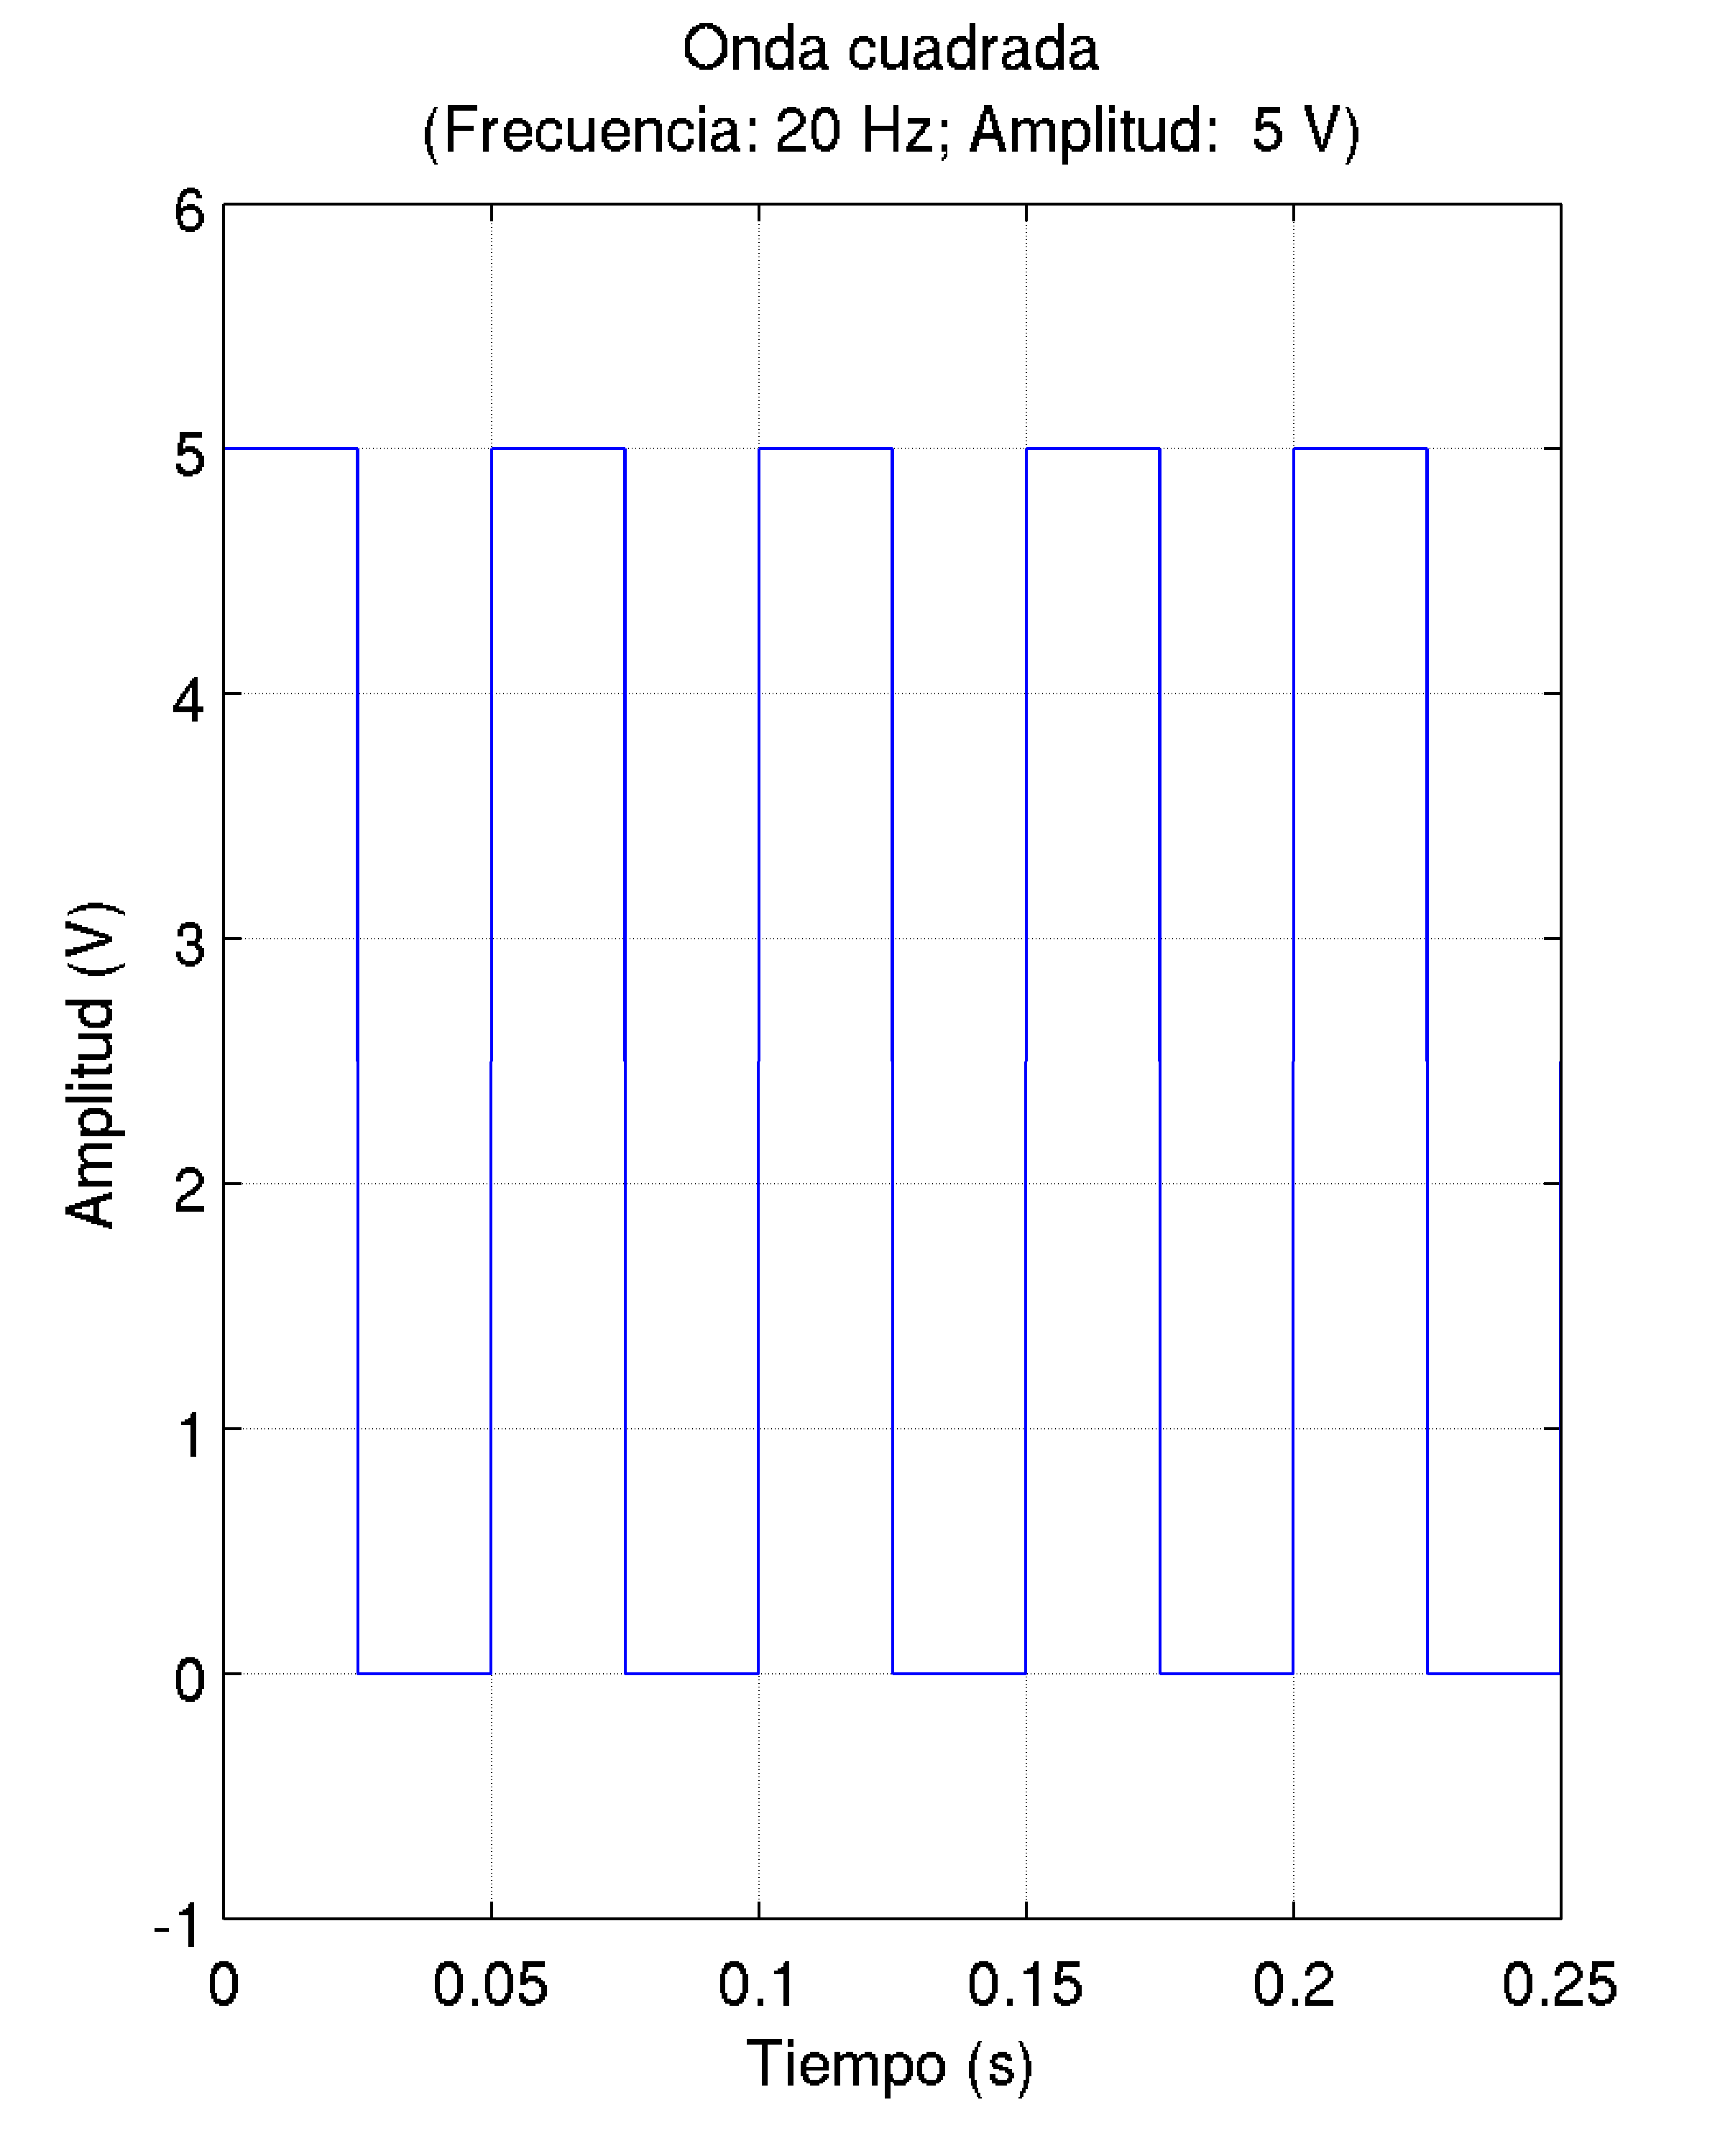
\includegraphics[height=5in]{./laboratorio_2/problema03_a.png}
      \end{figure}
      \vspace{\fill}

      \newpage
      \begin{listing}[H]
        \caption{Función de onda diente de sierra}
        \label{script03B}
        \inputminted{matlab}{./laboratorio_2/saww.m}
      \end{listing}

      \begin{figure}[H]
        \caption{Gráfico de la función rampa del \emph{script \ref{script03B}}.}
        \label{script03Bfigure}
        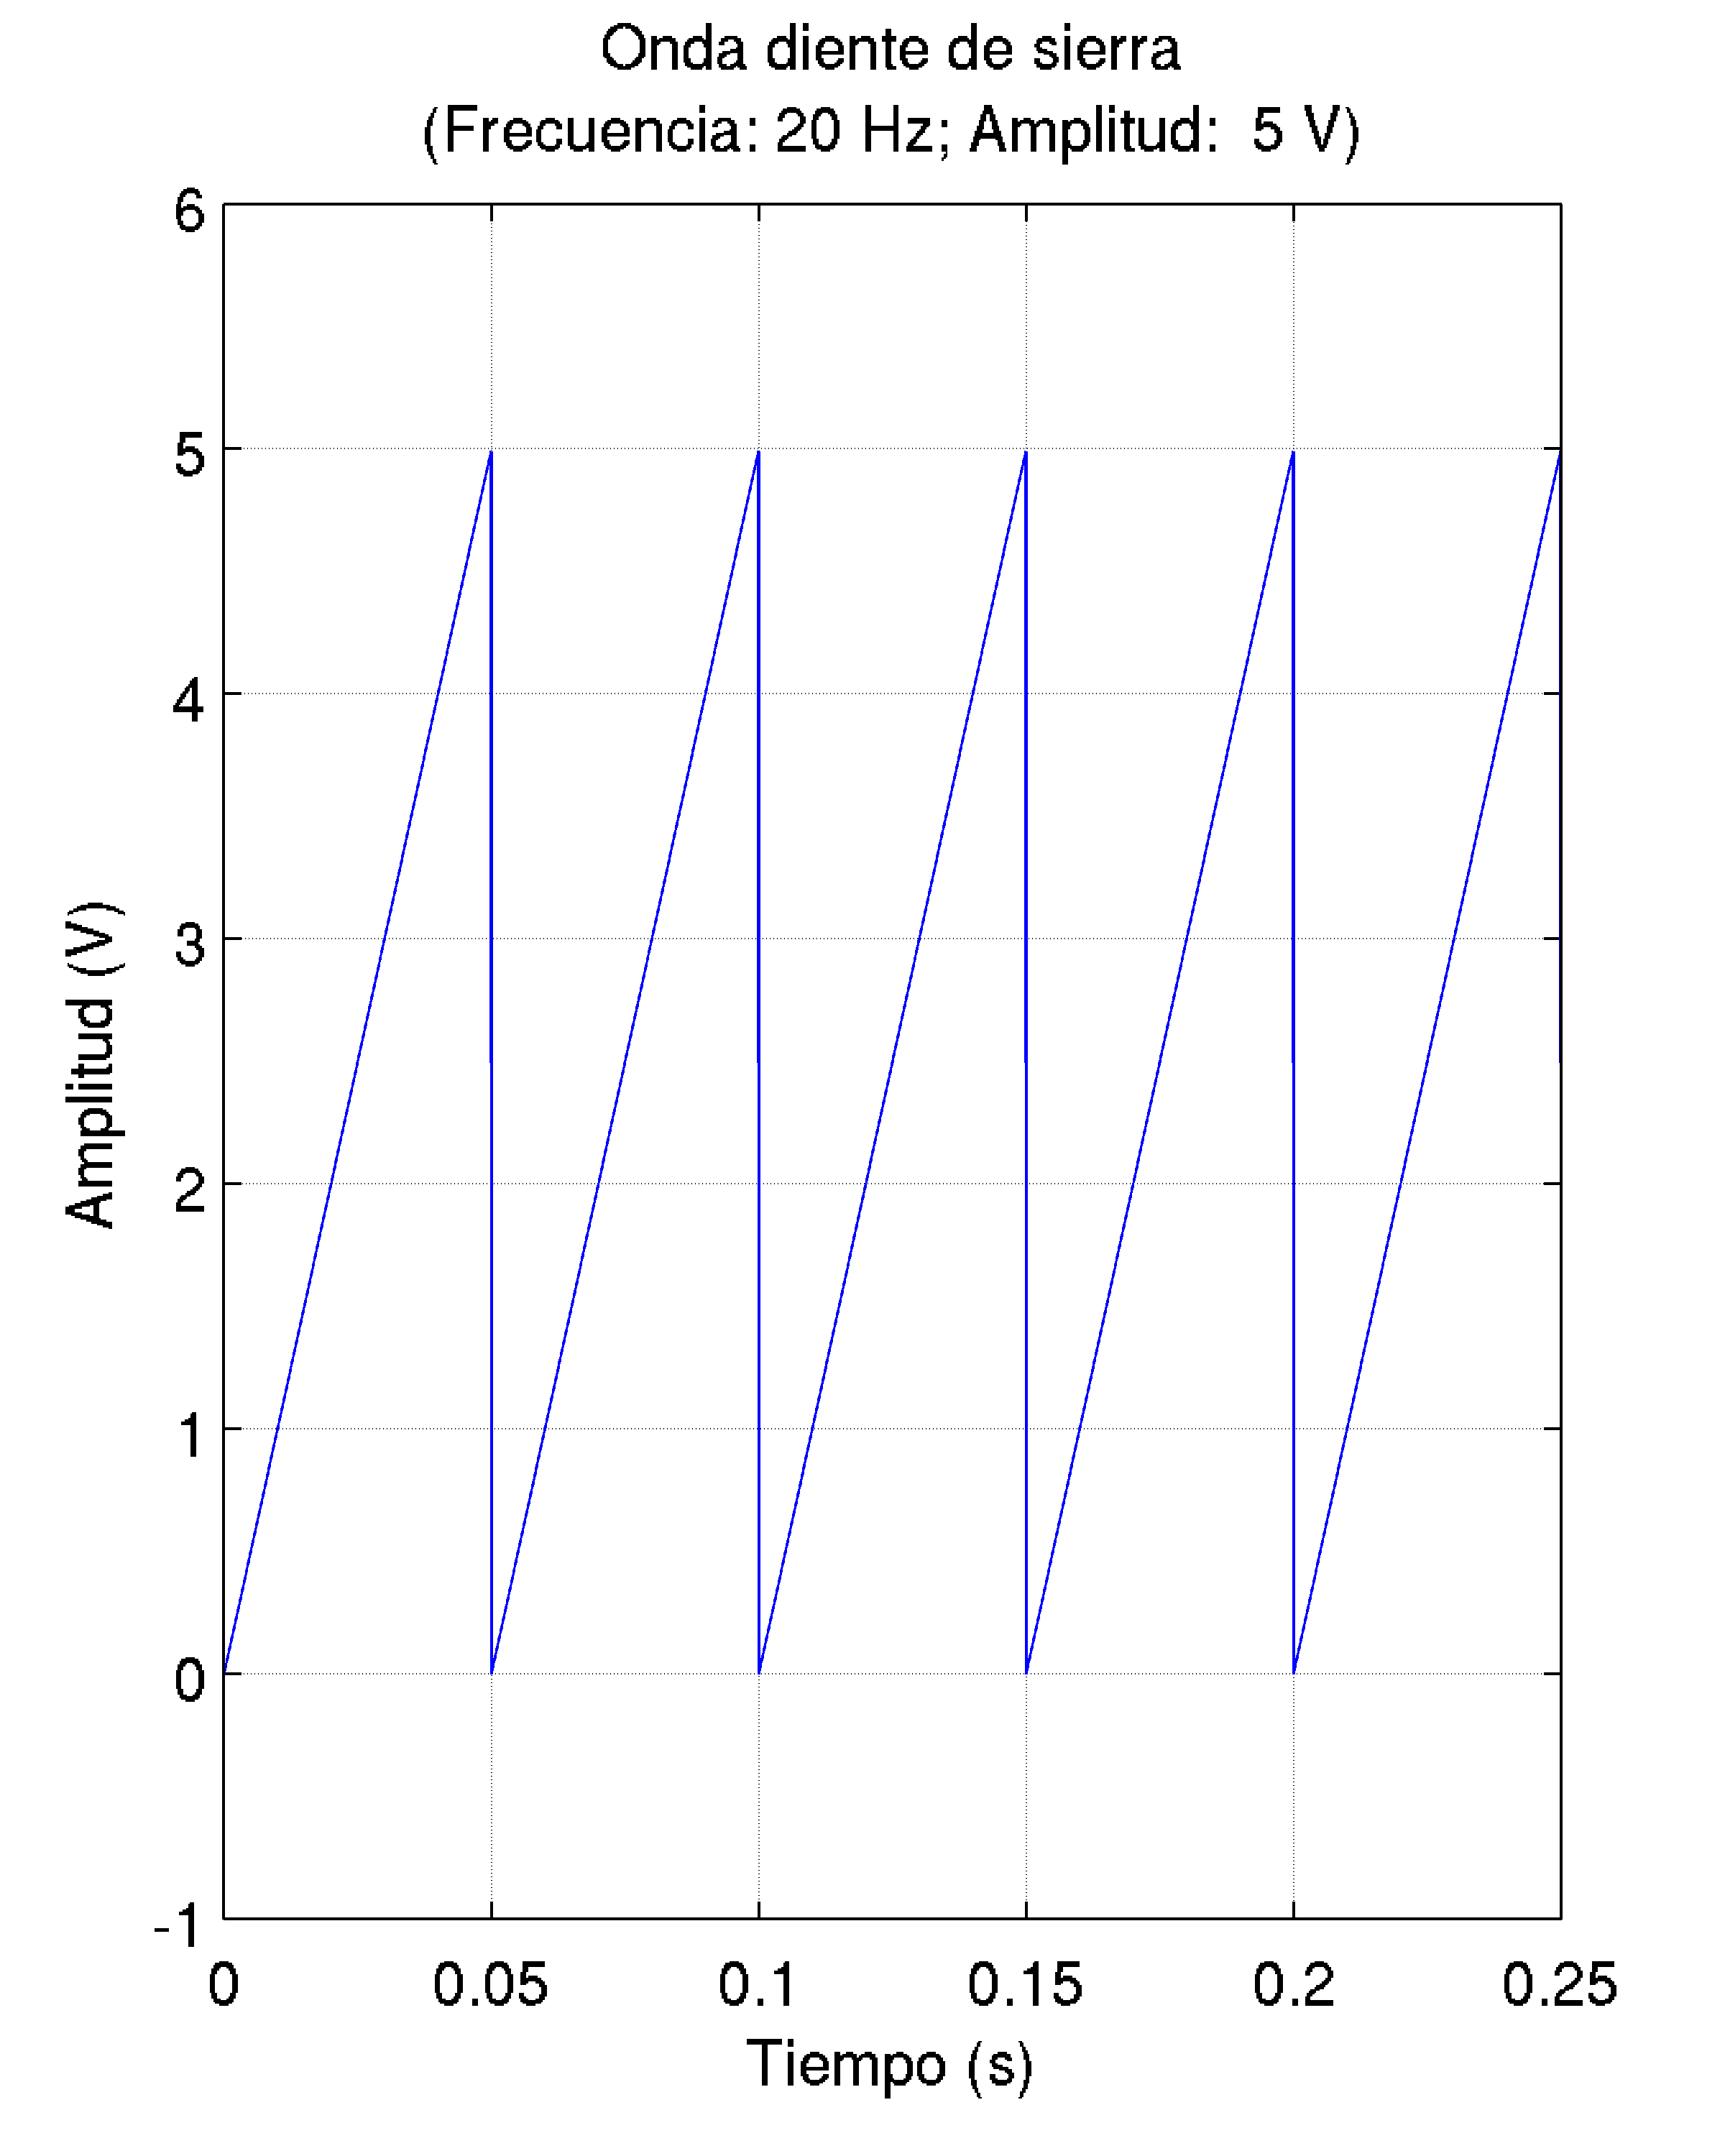
\includegraphics[height=5in]{./laboratorio_2/problema03_b.png}
      \end{figure}
      \vspace{\fill}

  \newpage
  \subsection*{Problema 4}
    \noindent La solución a una ecuación diferencial está dada por:
    $$x\left(x\right) = 10\mathrm{e}^{-t} - 5\mathrm{e}^{-0.5t}$$
    Usando \textsc{Matlab}, grafique la solución de la ecuación en el intervalo
    $I=\left[0,5\right]$ con una frecuencia de muestreo de 100 Hz.

    \subsubsection*{Solución}
      \begin{listing}[H]
        \caption{}
        \label{script04}
        \inputminted{matlab}{./laboratorio_2/problema04.m}
      \end{listing}

      \begin{figure}[H]
        \caption{Resultado de ejecutar el \emph{script \ref{script04}}.}
        \label{script04figure}
        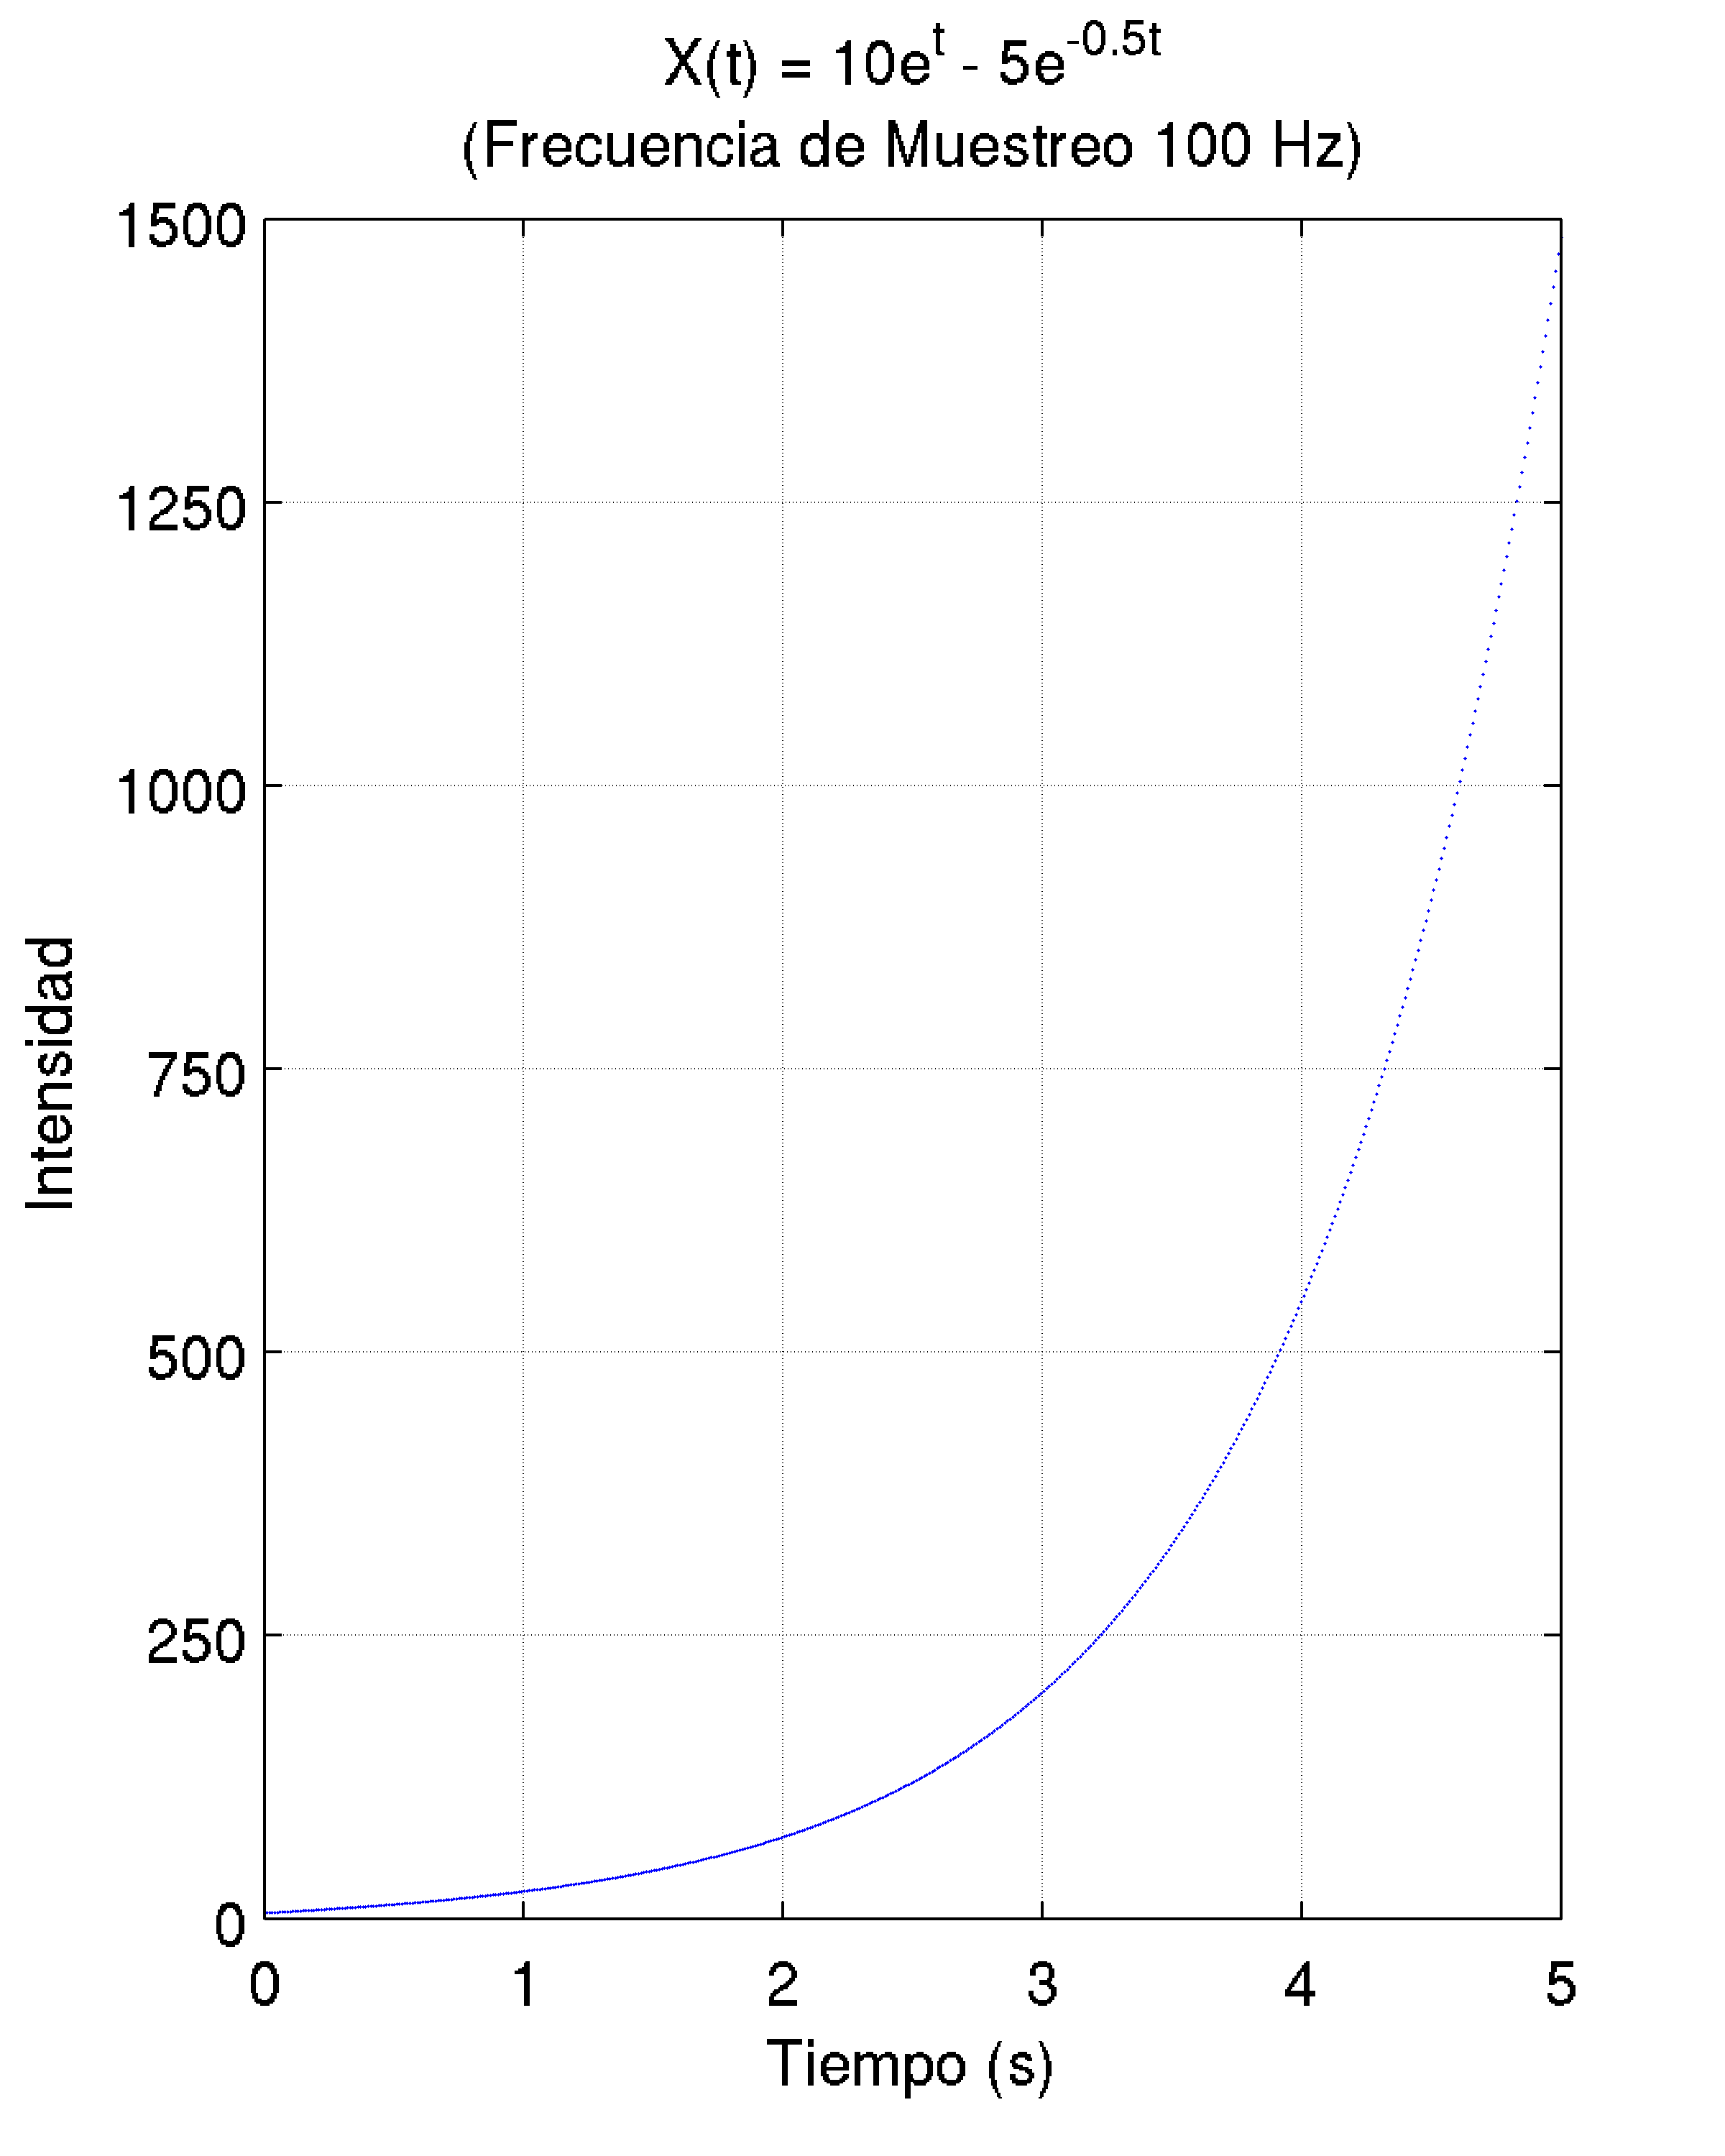
\includegraphics[height=5in]{./laboratorio_2/problema04.png}
      \end{figure}
      \vspace{\fill}

  \newpage
  \subsection*{Problema 5}
    \noindent Repita el problema anterior para la siguiente expresión:
    $$x\left(x\right) = 10\mathrm{e}^{-t} + 5\mathrm{e}^{-0.5t}$$

    \subsubsection*{Solución}
      \begin{listing}[H]
        \caption{}
        \label{script05}
        \inputminted{matlab}{./laboratorio_2/problema05.m}
      \end{listing}

      \begin{figure}[H]
        \caption{Resultado de ejecutar el \emph{script \ref{script05}}.}
        \label{script05figure}
        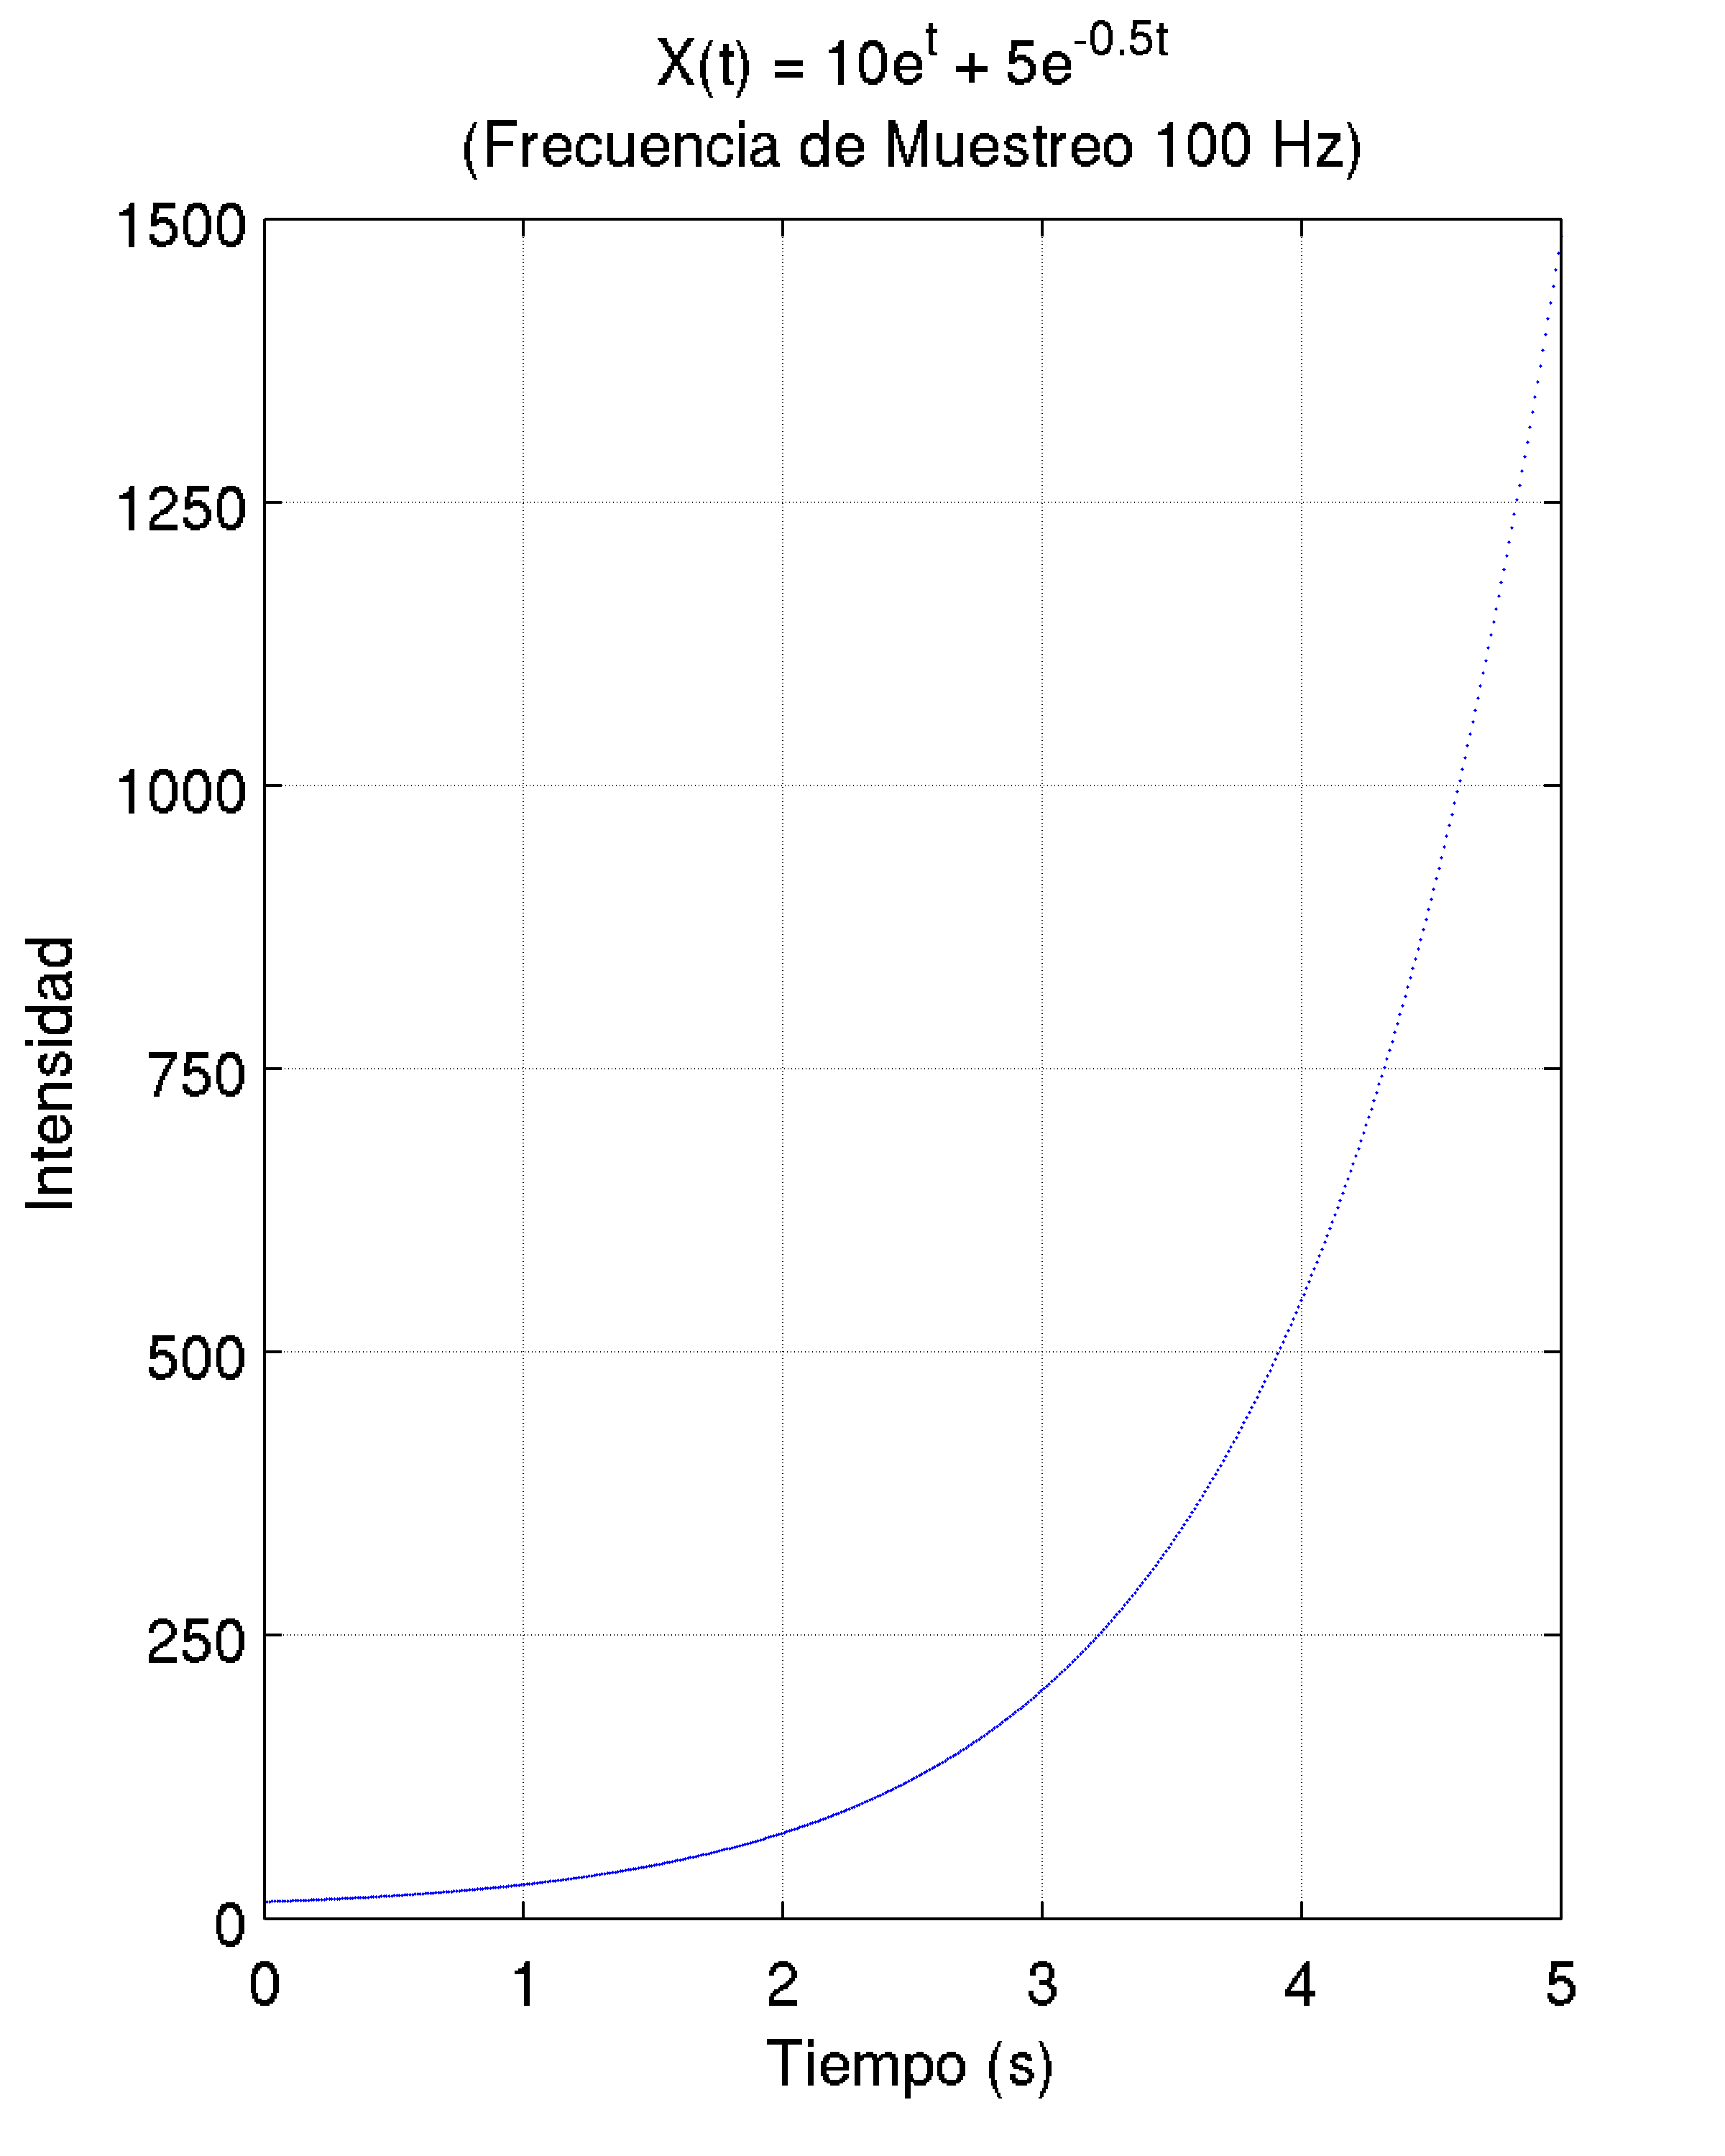
\includegraphics[height=5in]{./laboratorio_2/problema05.png}
      \end{figure}
      \vspace{\fill}

  \newpage
  \subsection*{Problema 6}
    \noindent Una señal sinusoidal con amortiguación exponencial está definida
    por la siguiente expresión:
    $$x\left(x\right) = \mathrm{e}^{-at}\cos\left(2\pi f t\right)$$
    donde $f = 1$ Hz y el parámetro $a$ es variable y toma valores sobre el
    siguiente conjunto: 1, 5, 20. Usando \textsc{Matlab}, investigar el
    efecto de variar dicho parámetro en la señal en el intervalo $[0, 5]$.
    Utilice una frecuencia de muestreo de 20 Hz. Calcule el valor de $a$
    para el caso de amortiguamiento crítico. Haga una gráfica para cada
    caso.

    \subsubsection*{Solución}
      \begin{listing}[H]
        \caption{}
        \label{script06}
        \inputminted{matlab}{./laboratorio_2/problema06.m}
      \end{listing}

      \begin{figure}[H]
        \caption{Resultado de ejecutar el \emph{script \ref{script06}}.}
        \label{script06figure}
        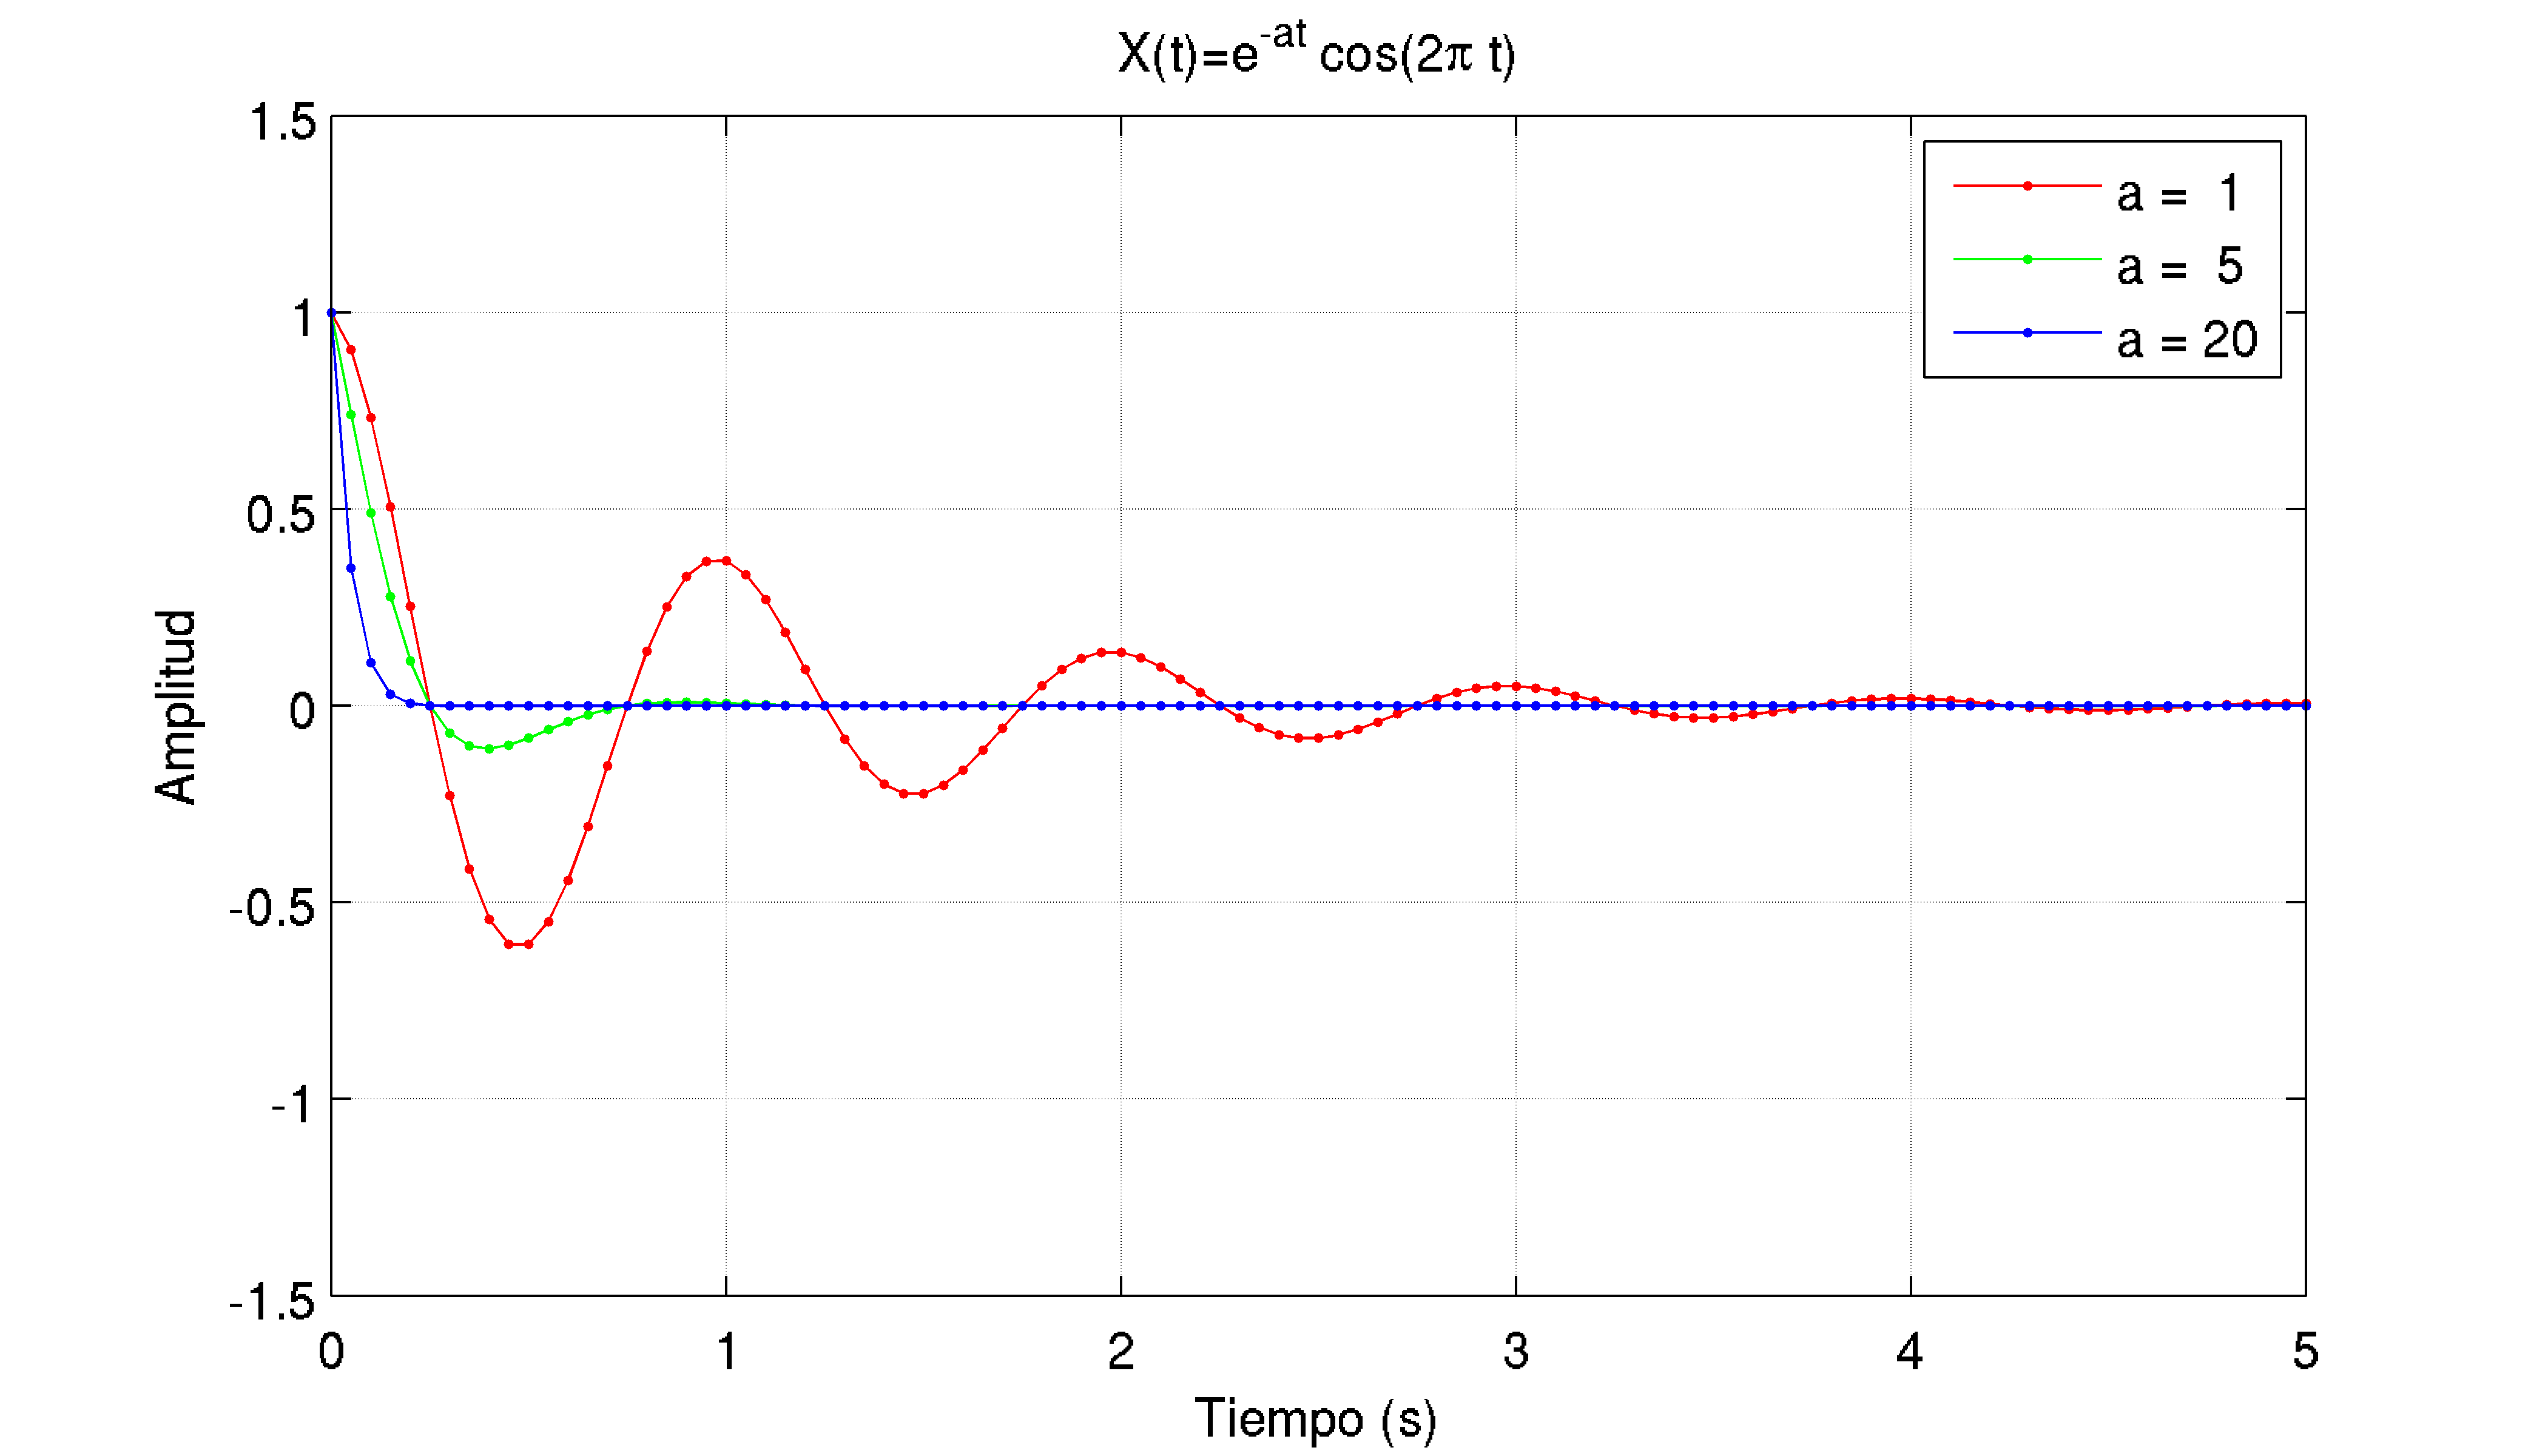
\includegraphics[width=0.9\textwidth]{./laboratorio_2/problema06.png}
      \end{figure}
      \vspace{\fill}
      \newpage
      \noindent De la ecuacion del oscilador amortiguado:
      $$ m \frac{\mathrm{d}^{2}x}{\mathrm{d}t^2} + b \frac{\mathrm{d}^{2}x}{\mathrm{d}t^2} + kx = 0. $$

      \noindent Para el caso con amortiguamiento débil, $b^2 < 4km$, la solución es de la forma
      $$ x\left(t\right) = x_0 \mathrm{e}^{-\frac{b}{2m}}\cos\left(\omega t\right). $$

      \noindent Comparando esta última expresión con la ecuación dada en
      el enunciado del problema, podemos identificar los términos:

      $$a = \frac{b}{2m}$$

      \noindent y

      $$\omega = \sqrt{\frac{k}{m} - \left(\frac{b}{2m}\right)^2} = 2\pi . $$

      \noindent Para el caso de amortiguamiento crítico se tiene que cumplir la
      condición $b = 4km$ de modo que
      $$ a^2_c = \frac{k}{m} $$
      \noindent Despejando de $\omega$, para un valor dado de $a$ se tiene
      $$ a_c = \sqrt{4\pi^2 - a^2} $$
      \vspace{\fill}

  \newpage
  \subsection*{Problema 7}
    \noindent Para la gráfica mostrada, haga una función en Matlab que
    visualice $h(t)$. Use el comando \texttt{function}.

    \begin{figure}[H]
        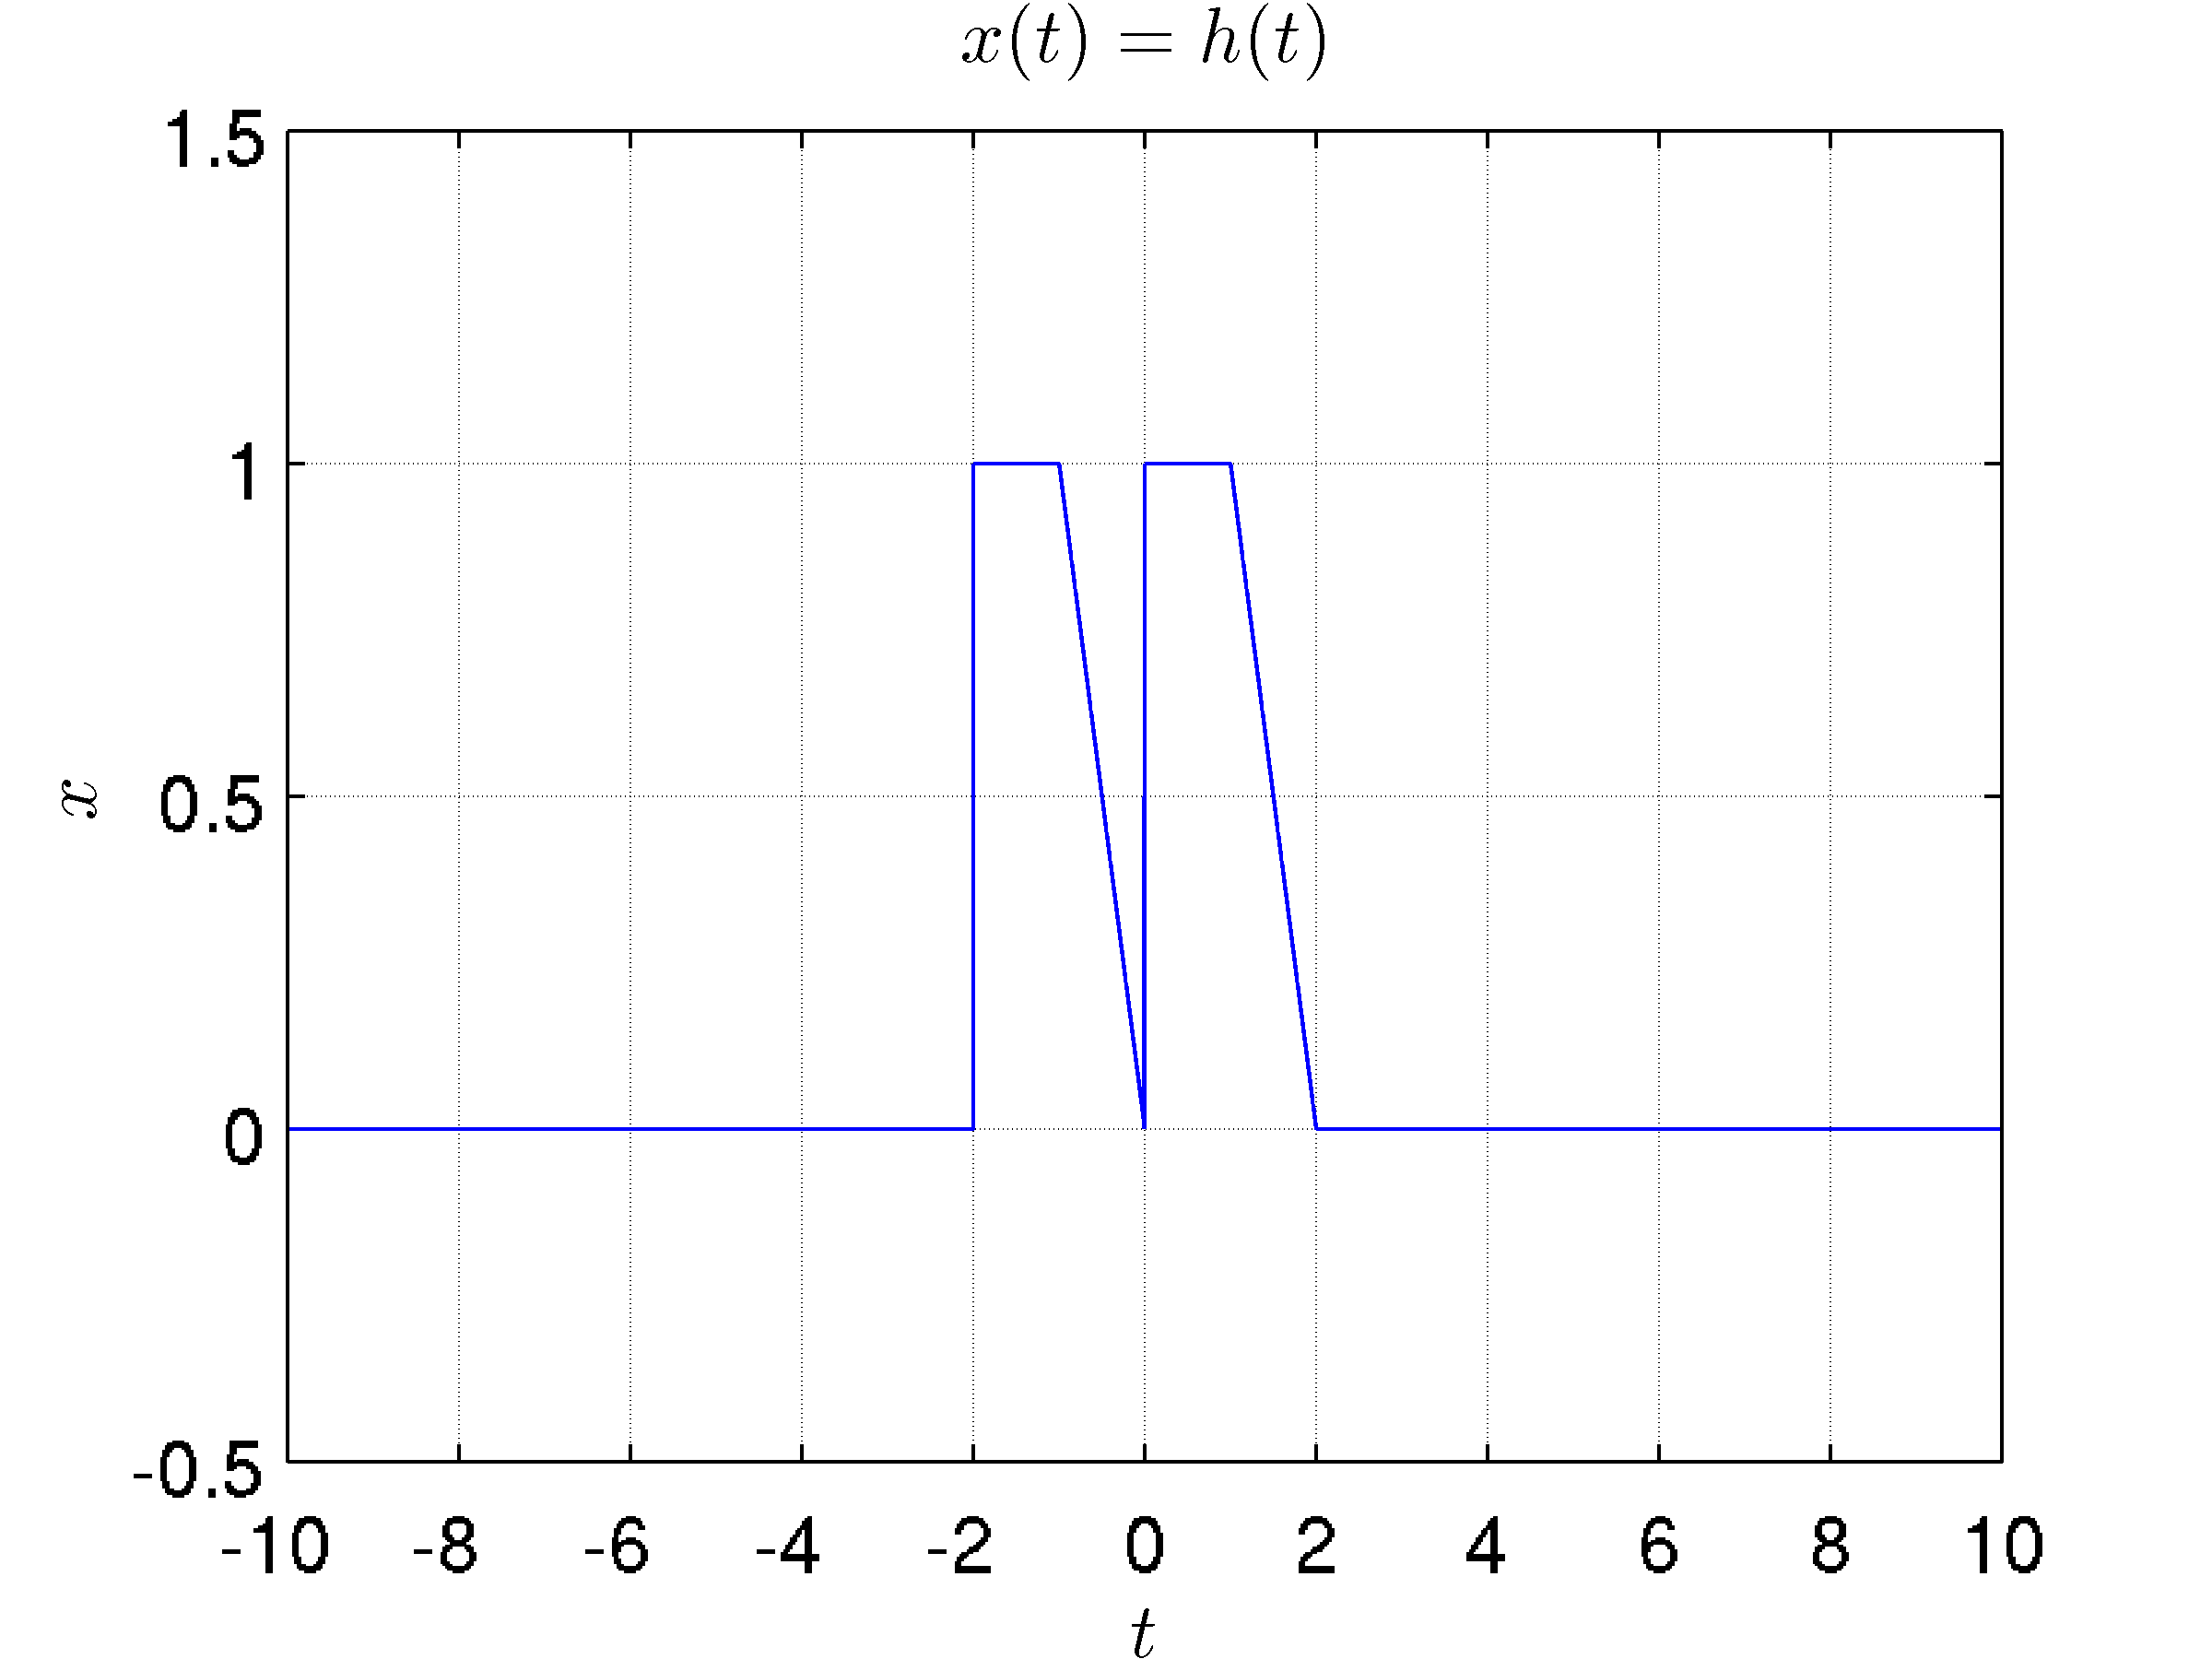
\includegraphics[width=4in]{./laboratorio_2/problema07.png}
    \end{figure}

    \noindent Graficar:
    \begin{enumerate}
        \item $h\left(t+1\right)$
        \item $h\left(\frac{t}{2}-2\right)$
        \item $h\left(1-2t\right)$
        \item $4h\left(\frac{t}{4}\right)$
        \item $\frac{1}{2}h\left(t\right)u\left(t\right) + h\left(-t\right)u\left(t\right)$
        \item $h\left(\frac{t}{2}\right)\delta\left(t+1\right)$
        \item $h\left(t\right)\left(u\left(t+1\right)-u\left(t-1\right)\right)$
    \end{enumerate}

    \subsubsection*{Solución}
      \begin{listing}[H]
        \caption{Función que replica la gráfica mostrada en el enunciado.}
        \label{script07}
        \inputminted{matlab}{./laboratorio_2/hfun.m}
      \end{listing}
      \vspace{\fill}

      \newpage
      \begin{listing}[H]
        \caption{Script para realizar los gráficos solicitados.}
        \label{script07A}
        \inputminted[firstline=5]{matlab}{./laboratorio_2/problema07.m}
      \end{listing}
      \vspace{\fill}

      \newpage
      \begin{figure}[H]
        \caption{Resultados de la ejecucion del \emph{script} \ref{script07A}.}
        \label{script07figure1}
        \vspace{0.7em}
        \vspace{0.1em}
        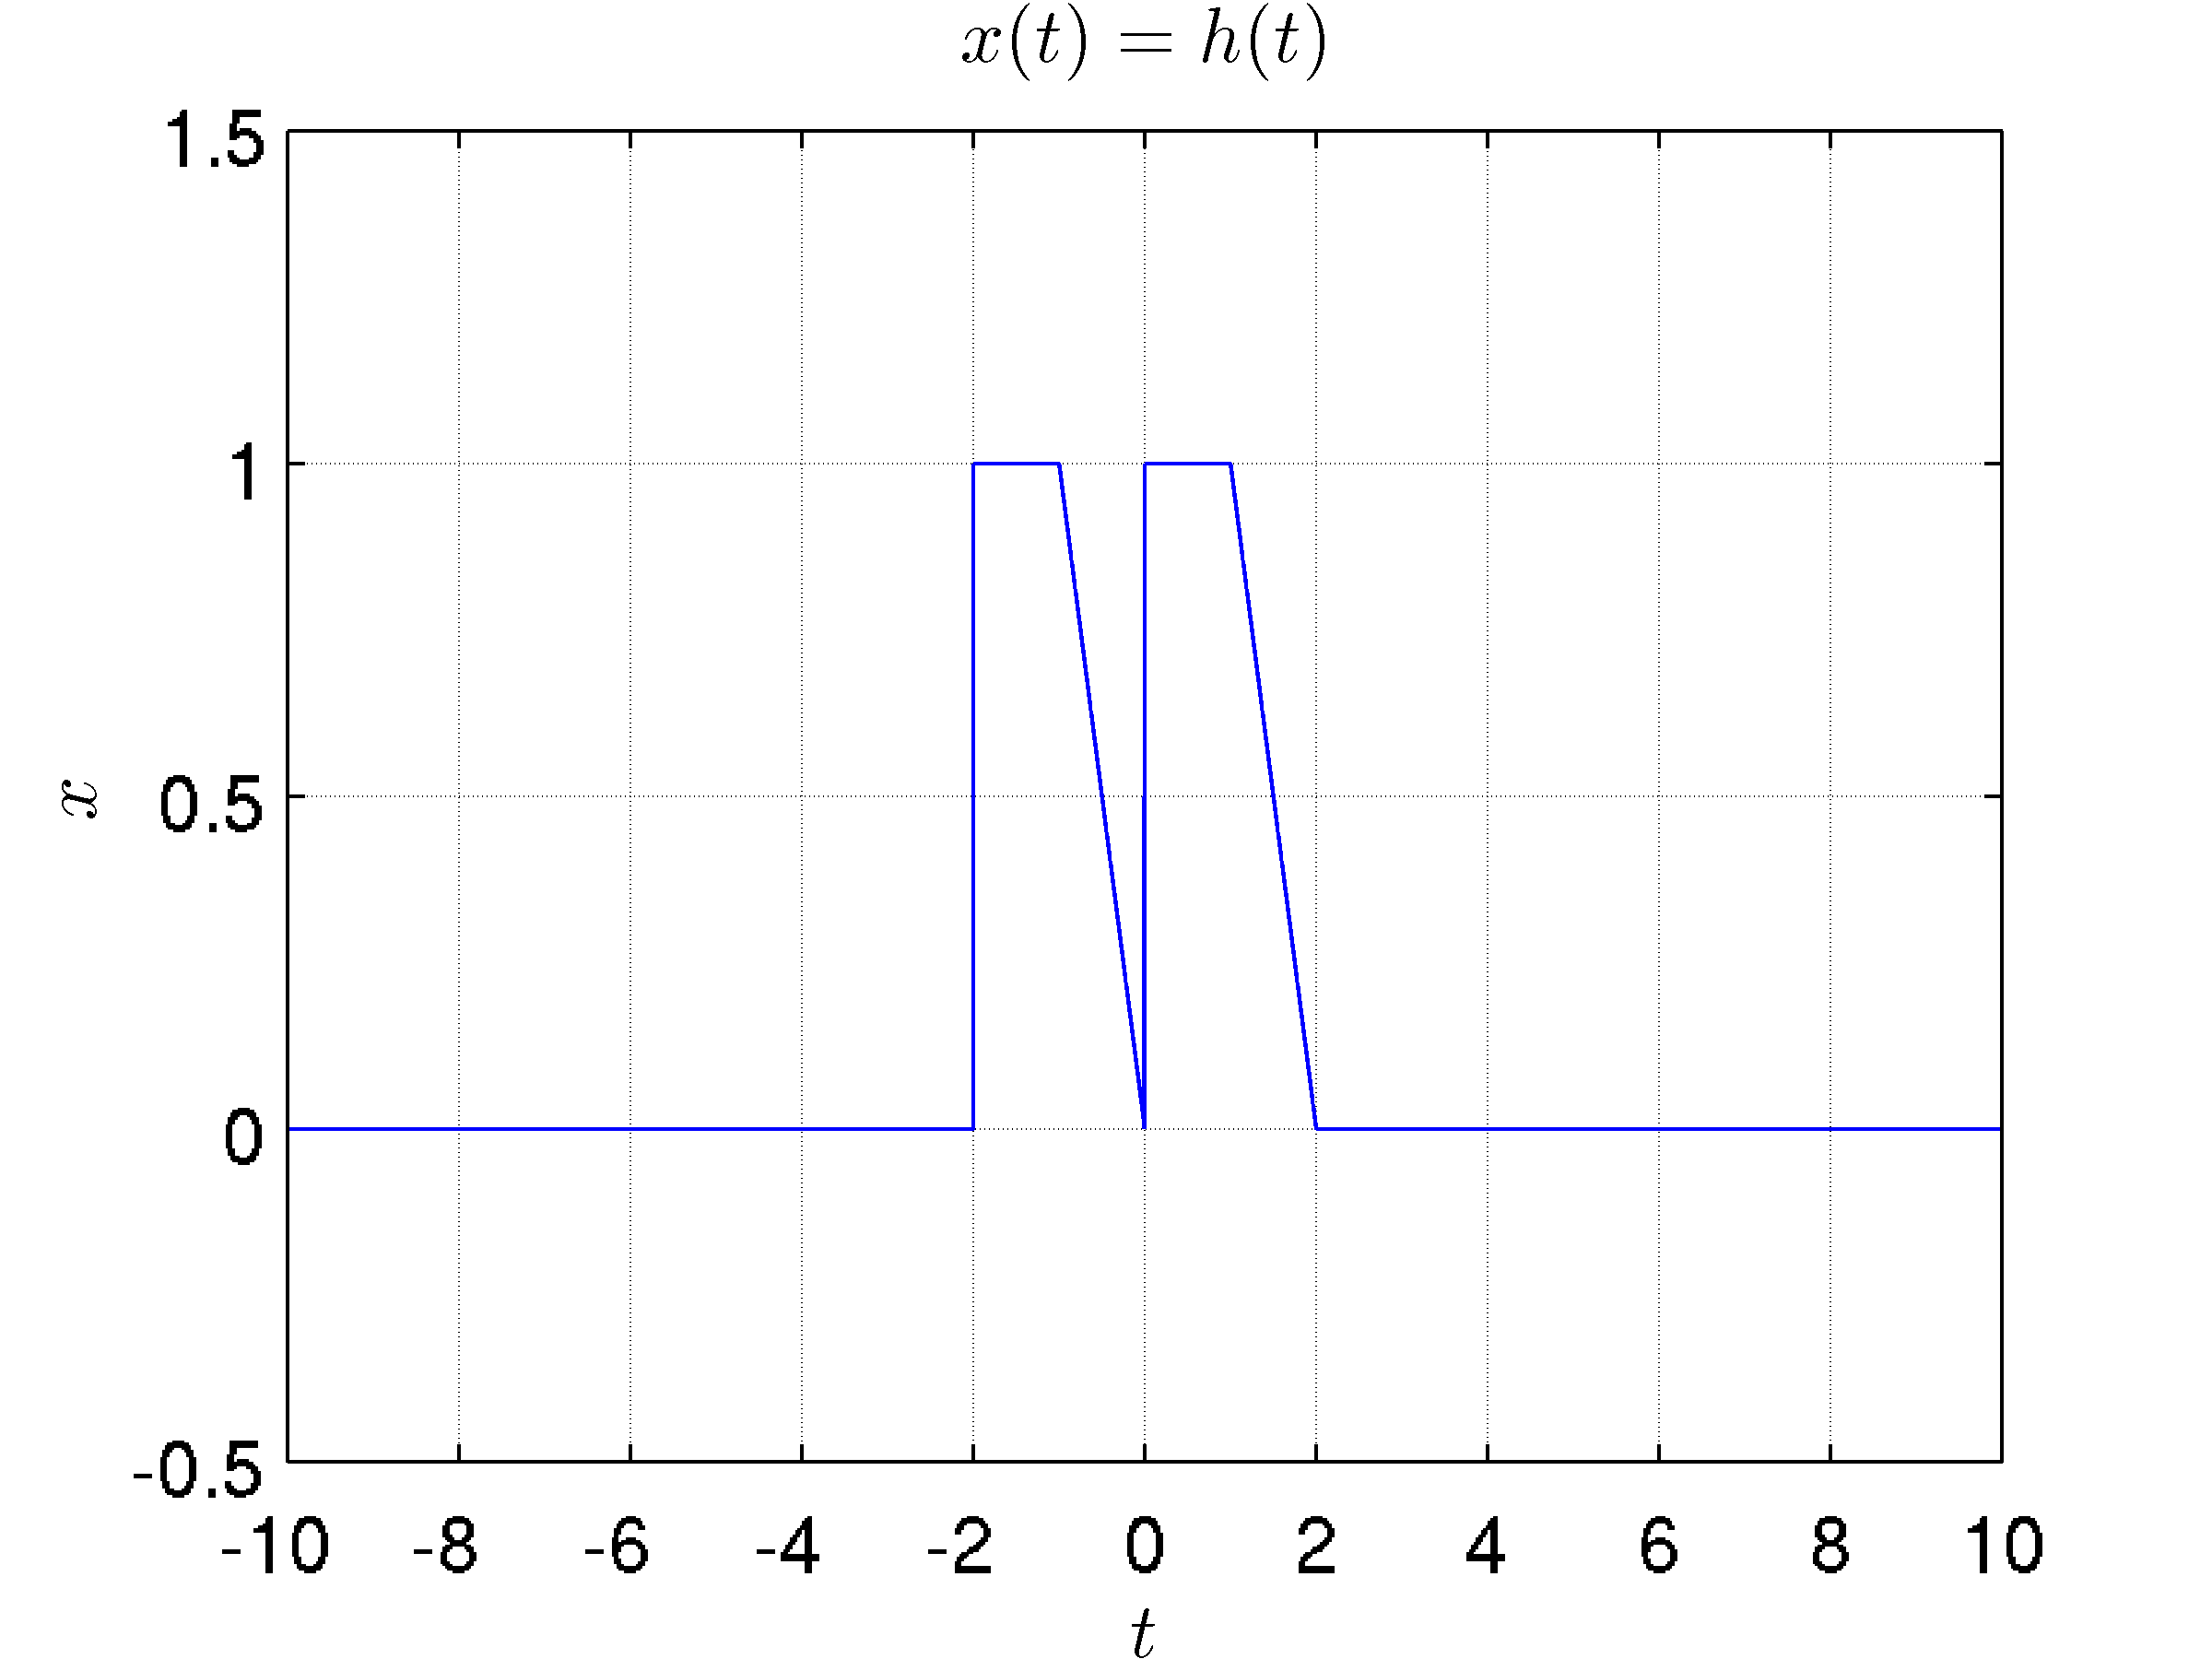
\includegraphics[width=3in]{./laboratorio_2/problema07.png}
        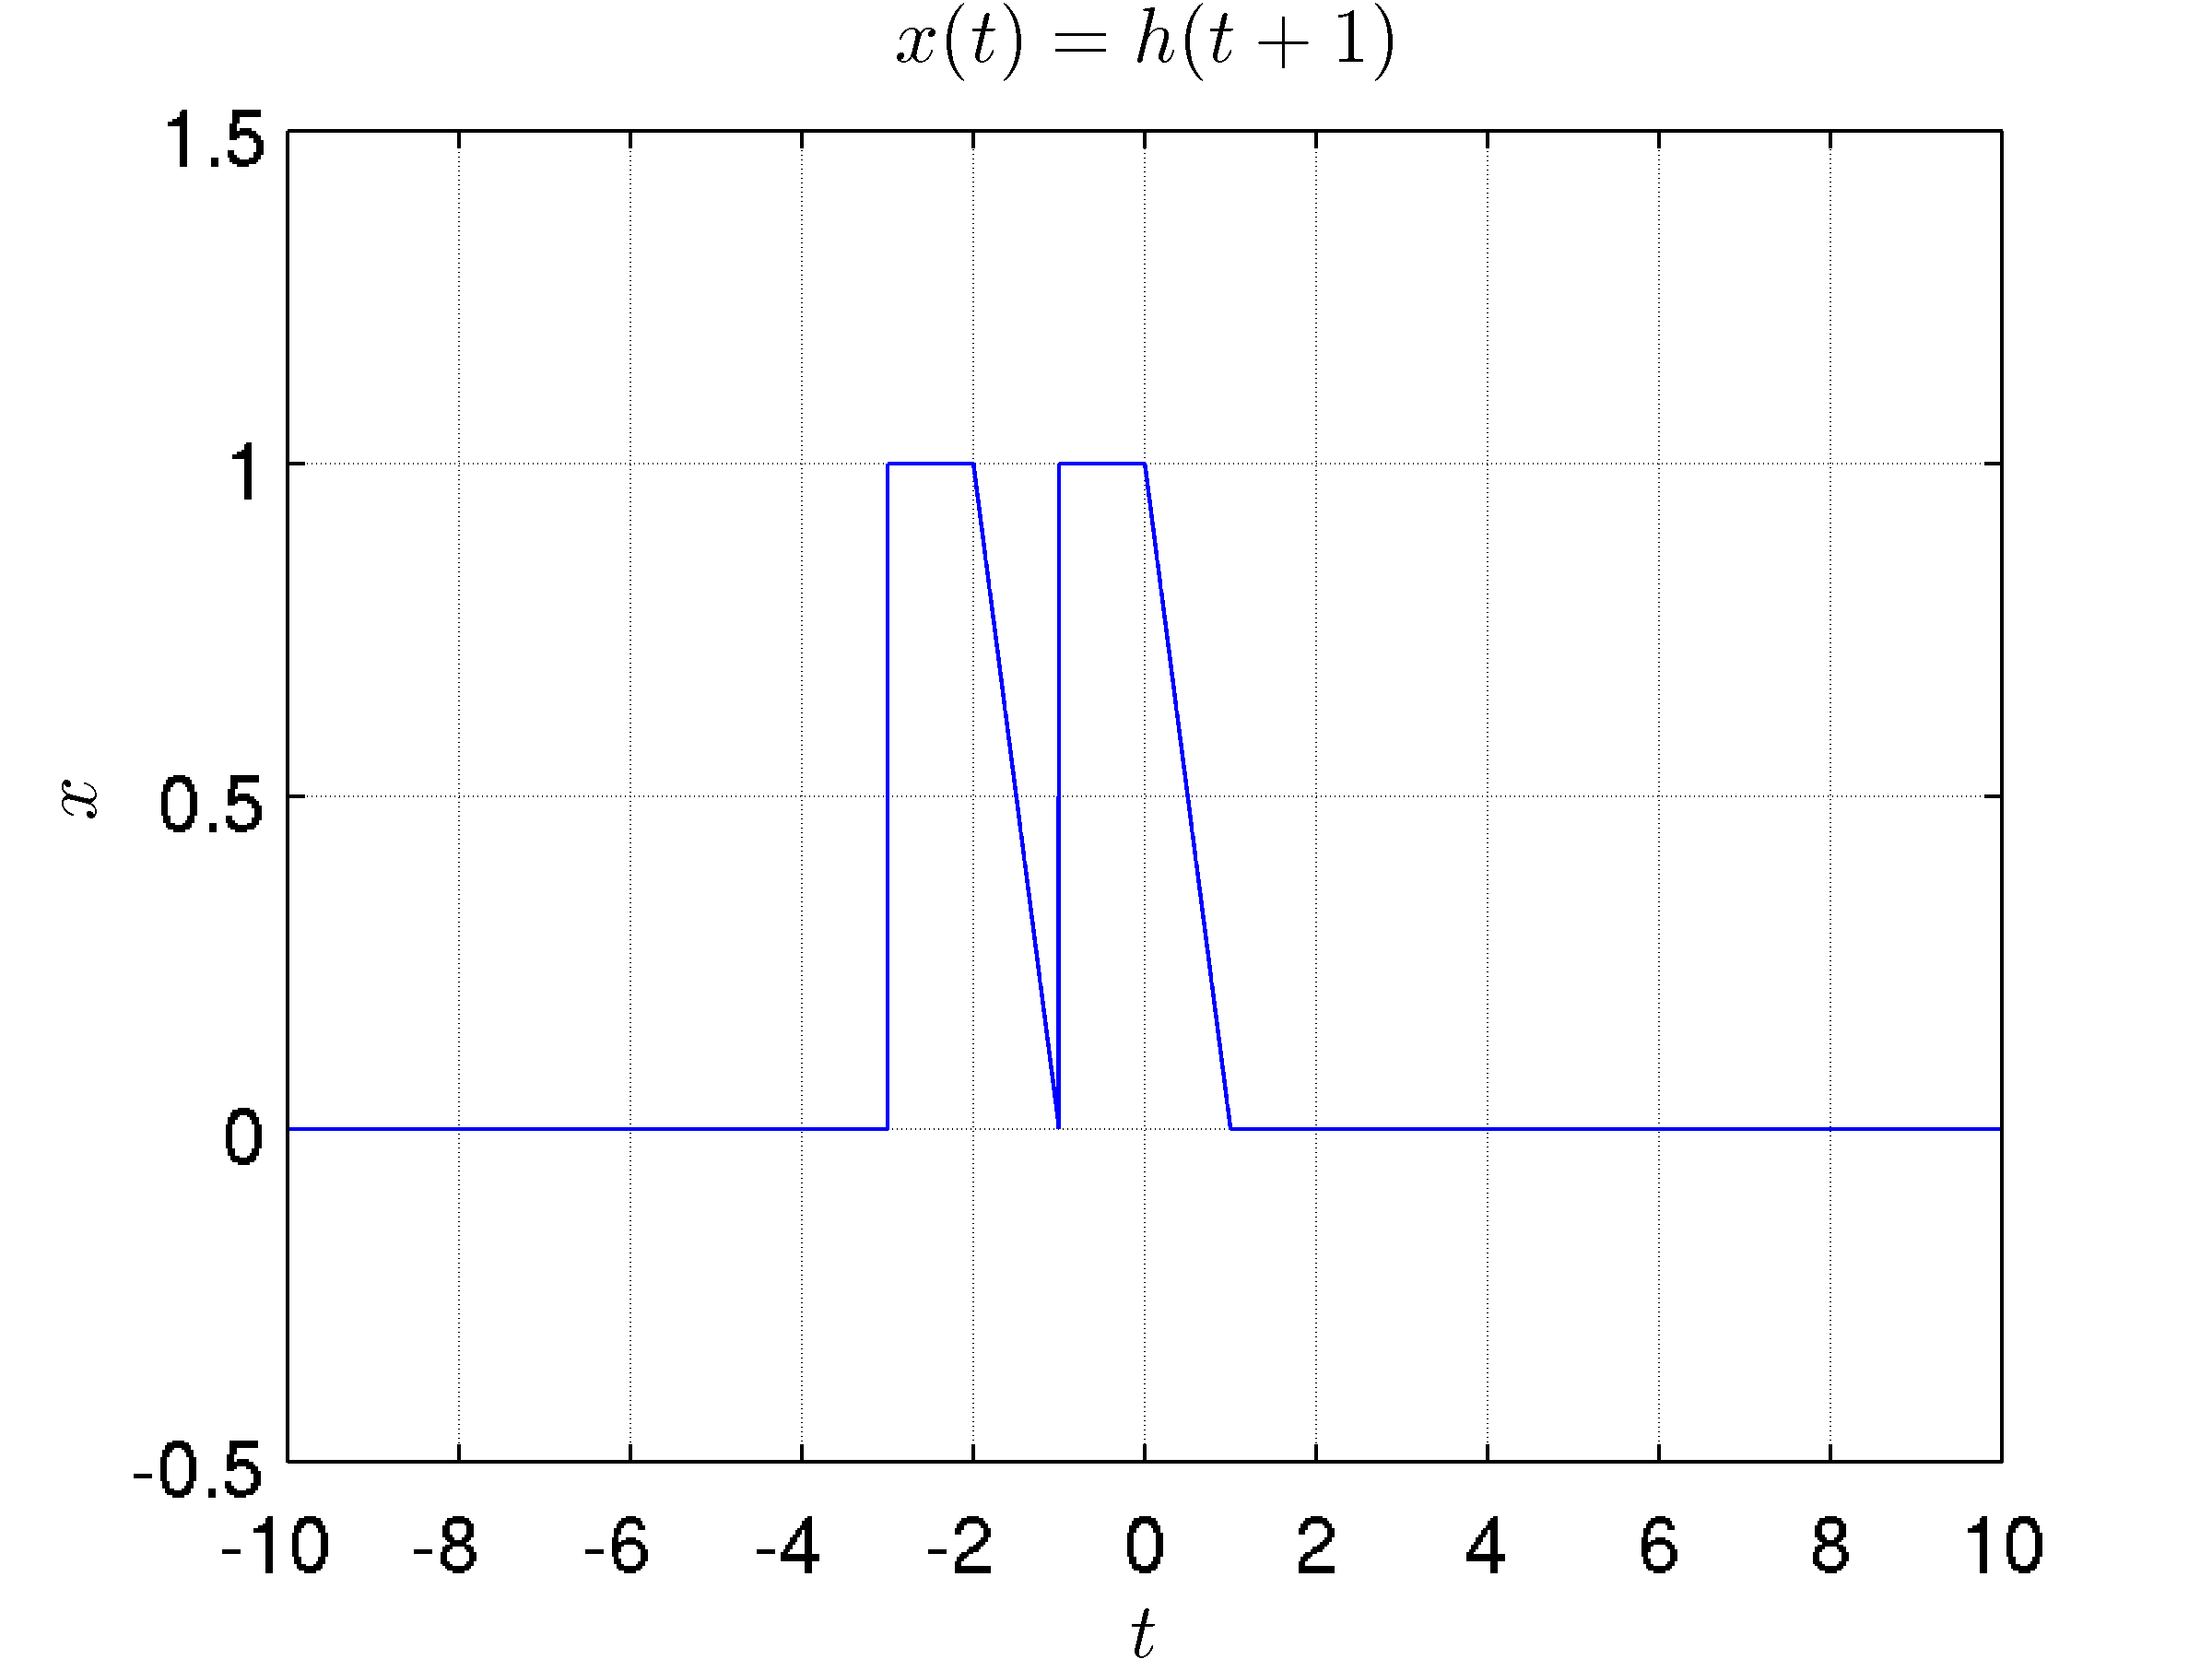
\includegraphics[width=3in]{./laboratorio_2/problema07_a.png}
        \vspace{0.7em}
        \vspace{0.1em}
        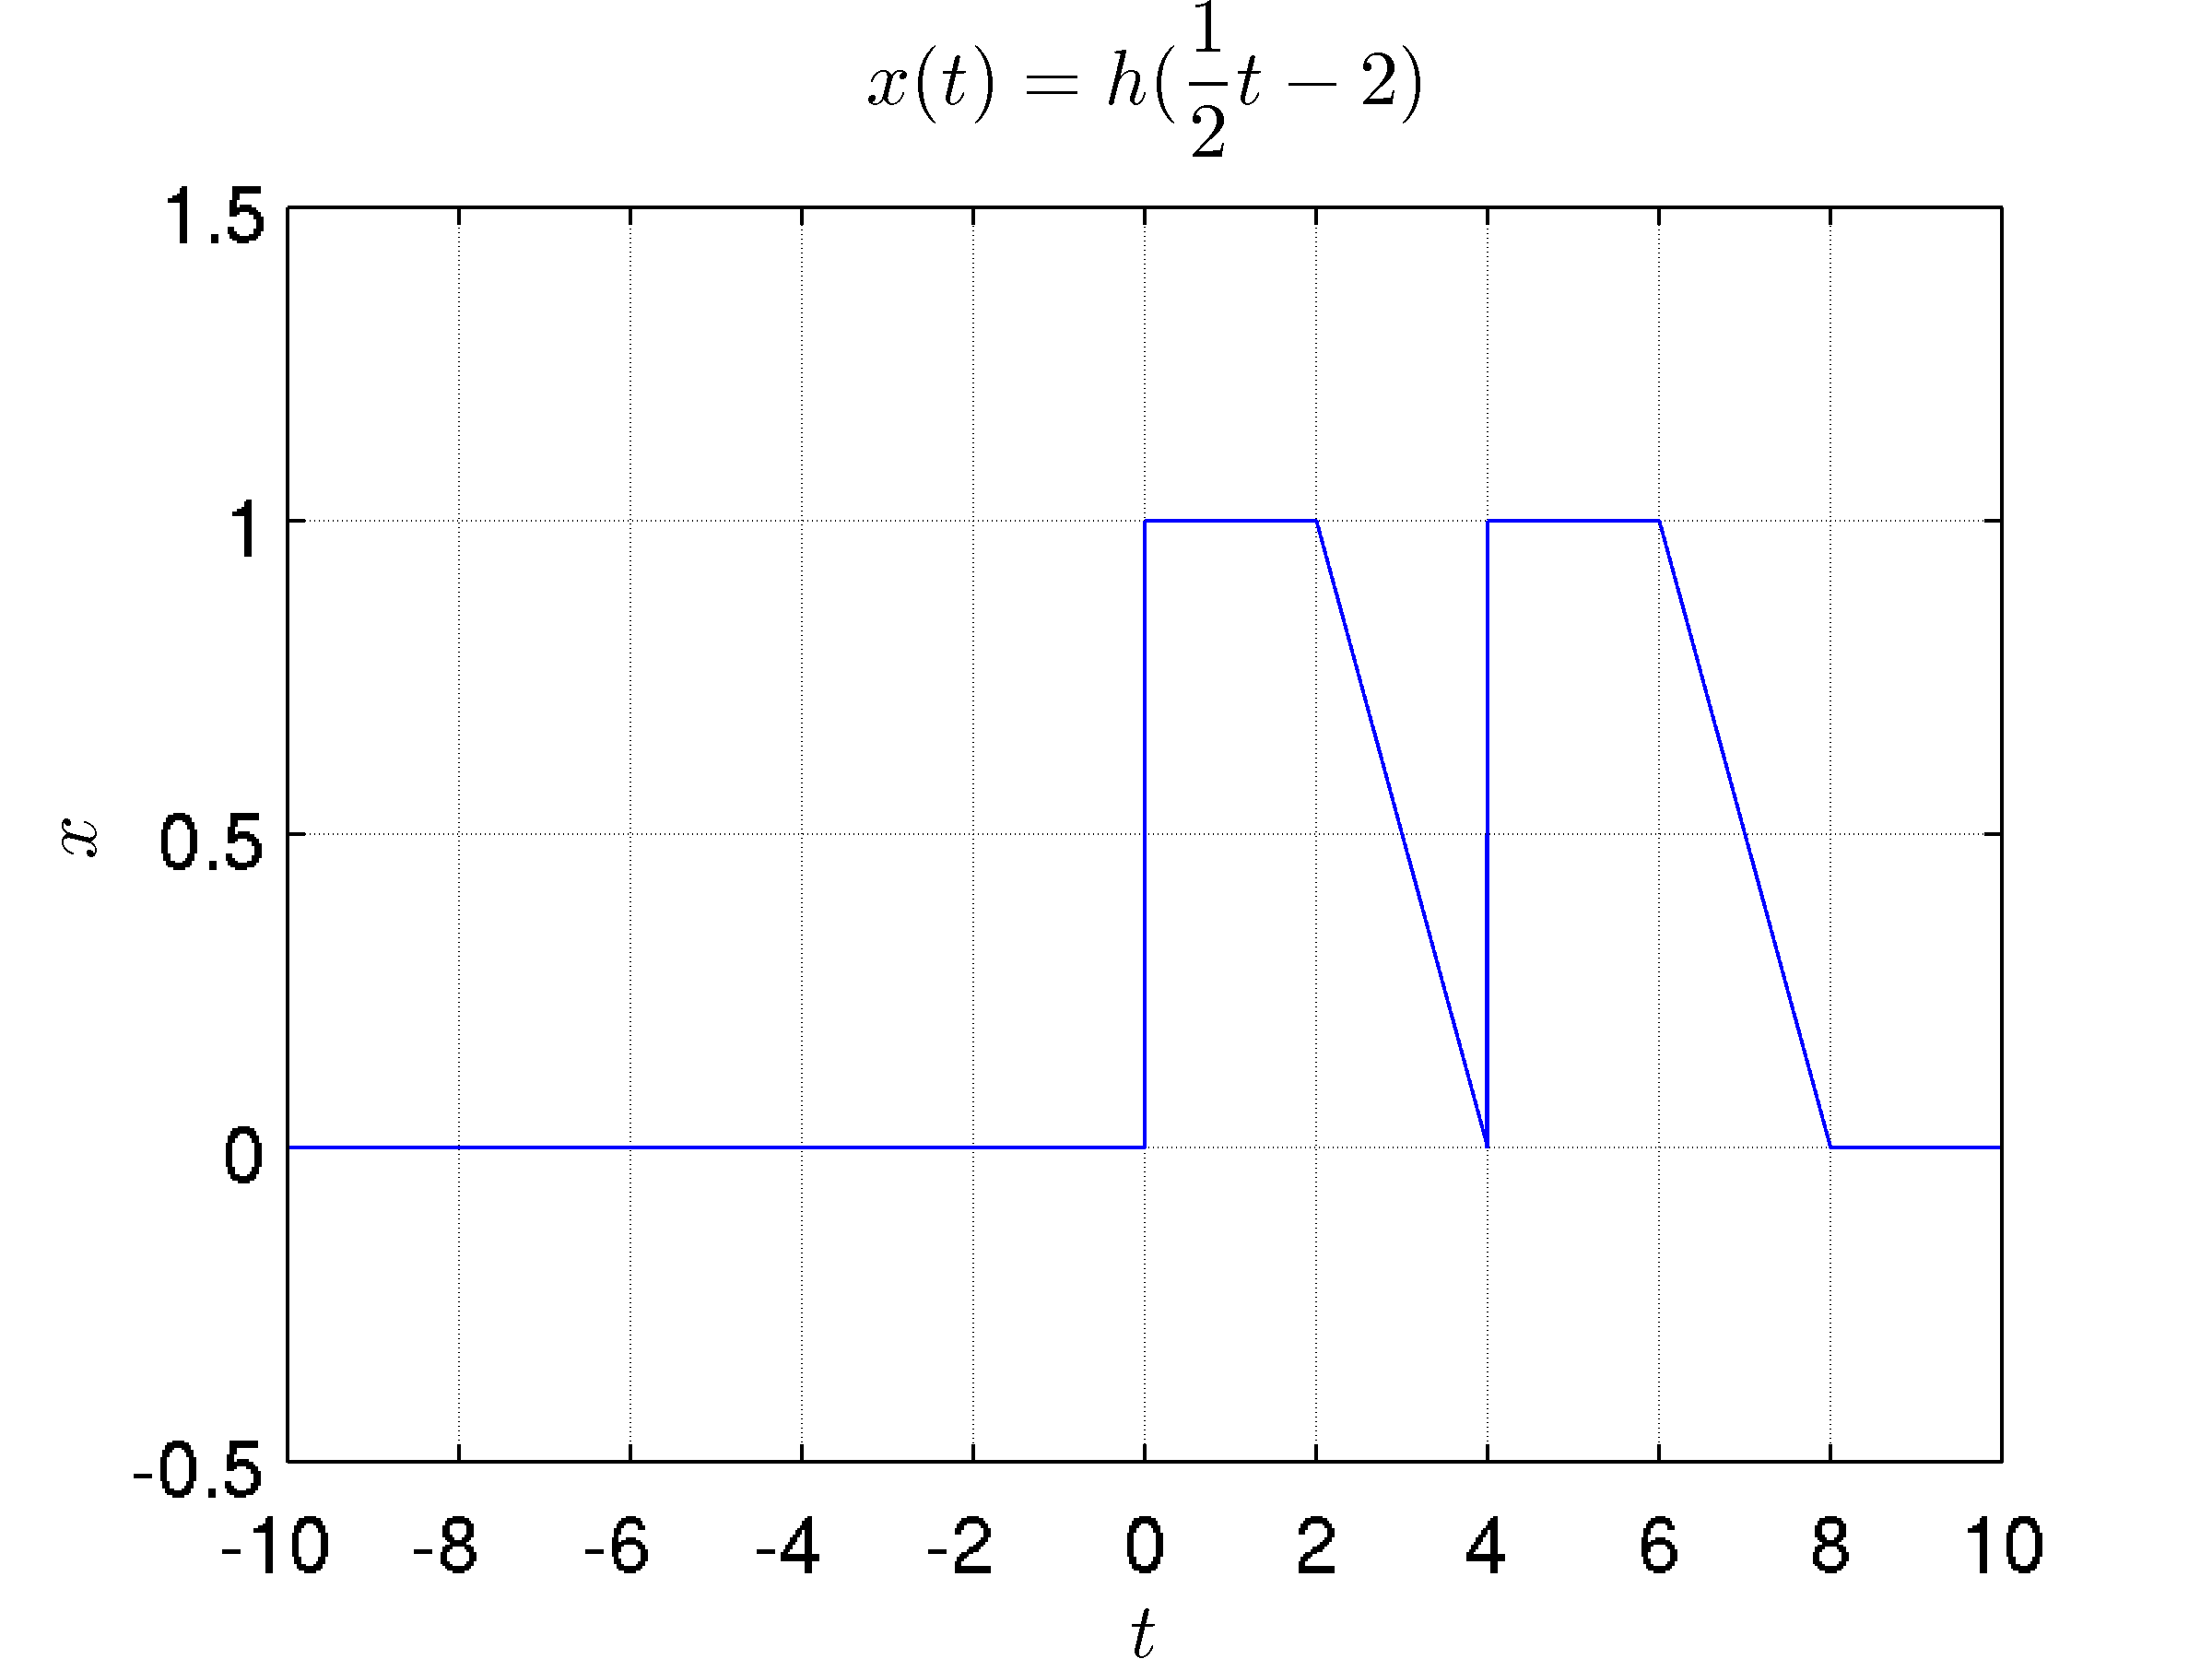
\includegraphics[width=3in]{./laboratorio_2/problema07_b.png}
        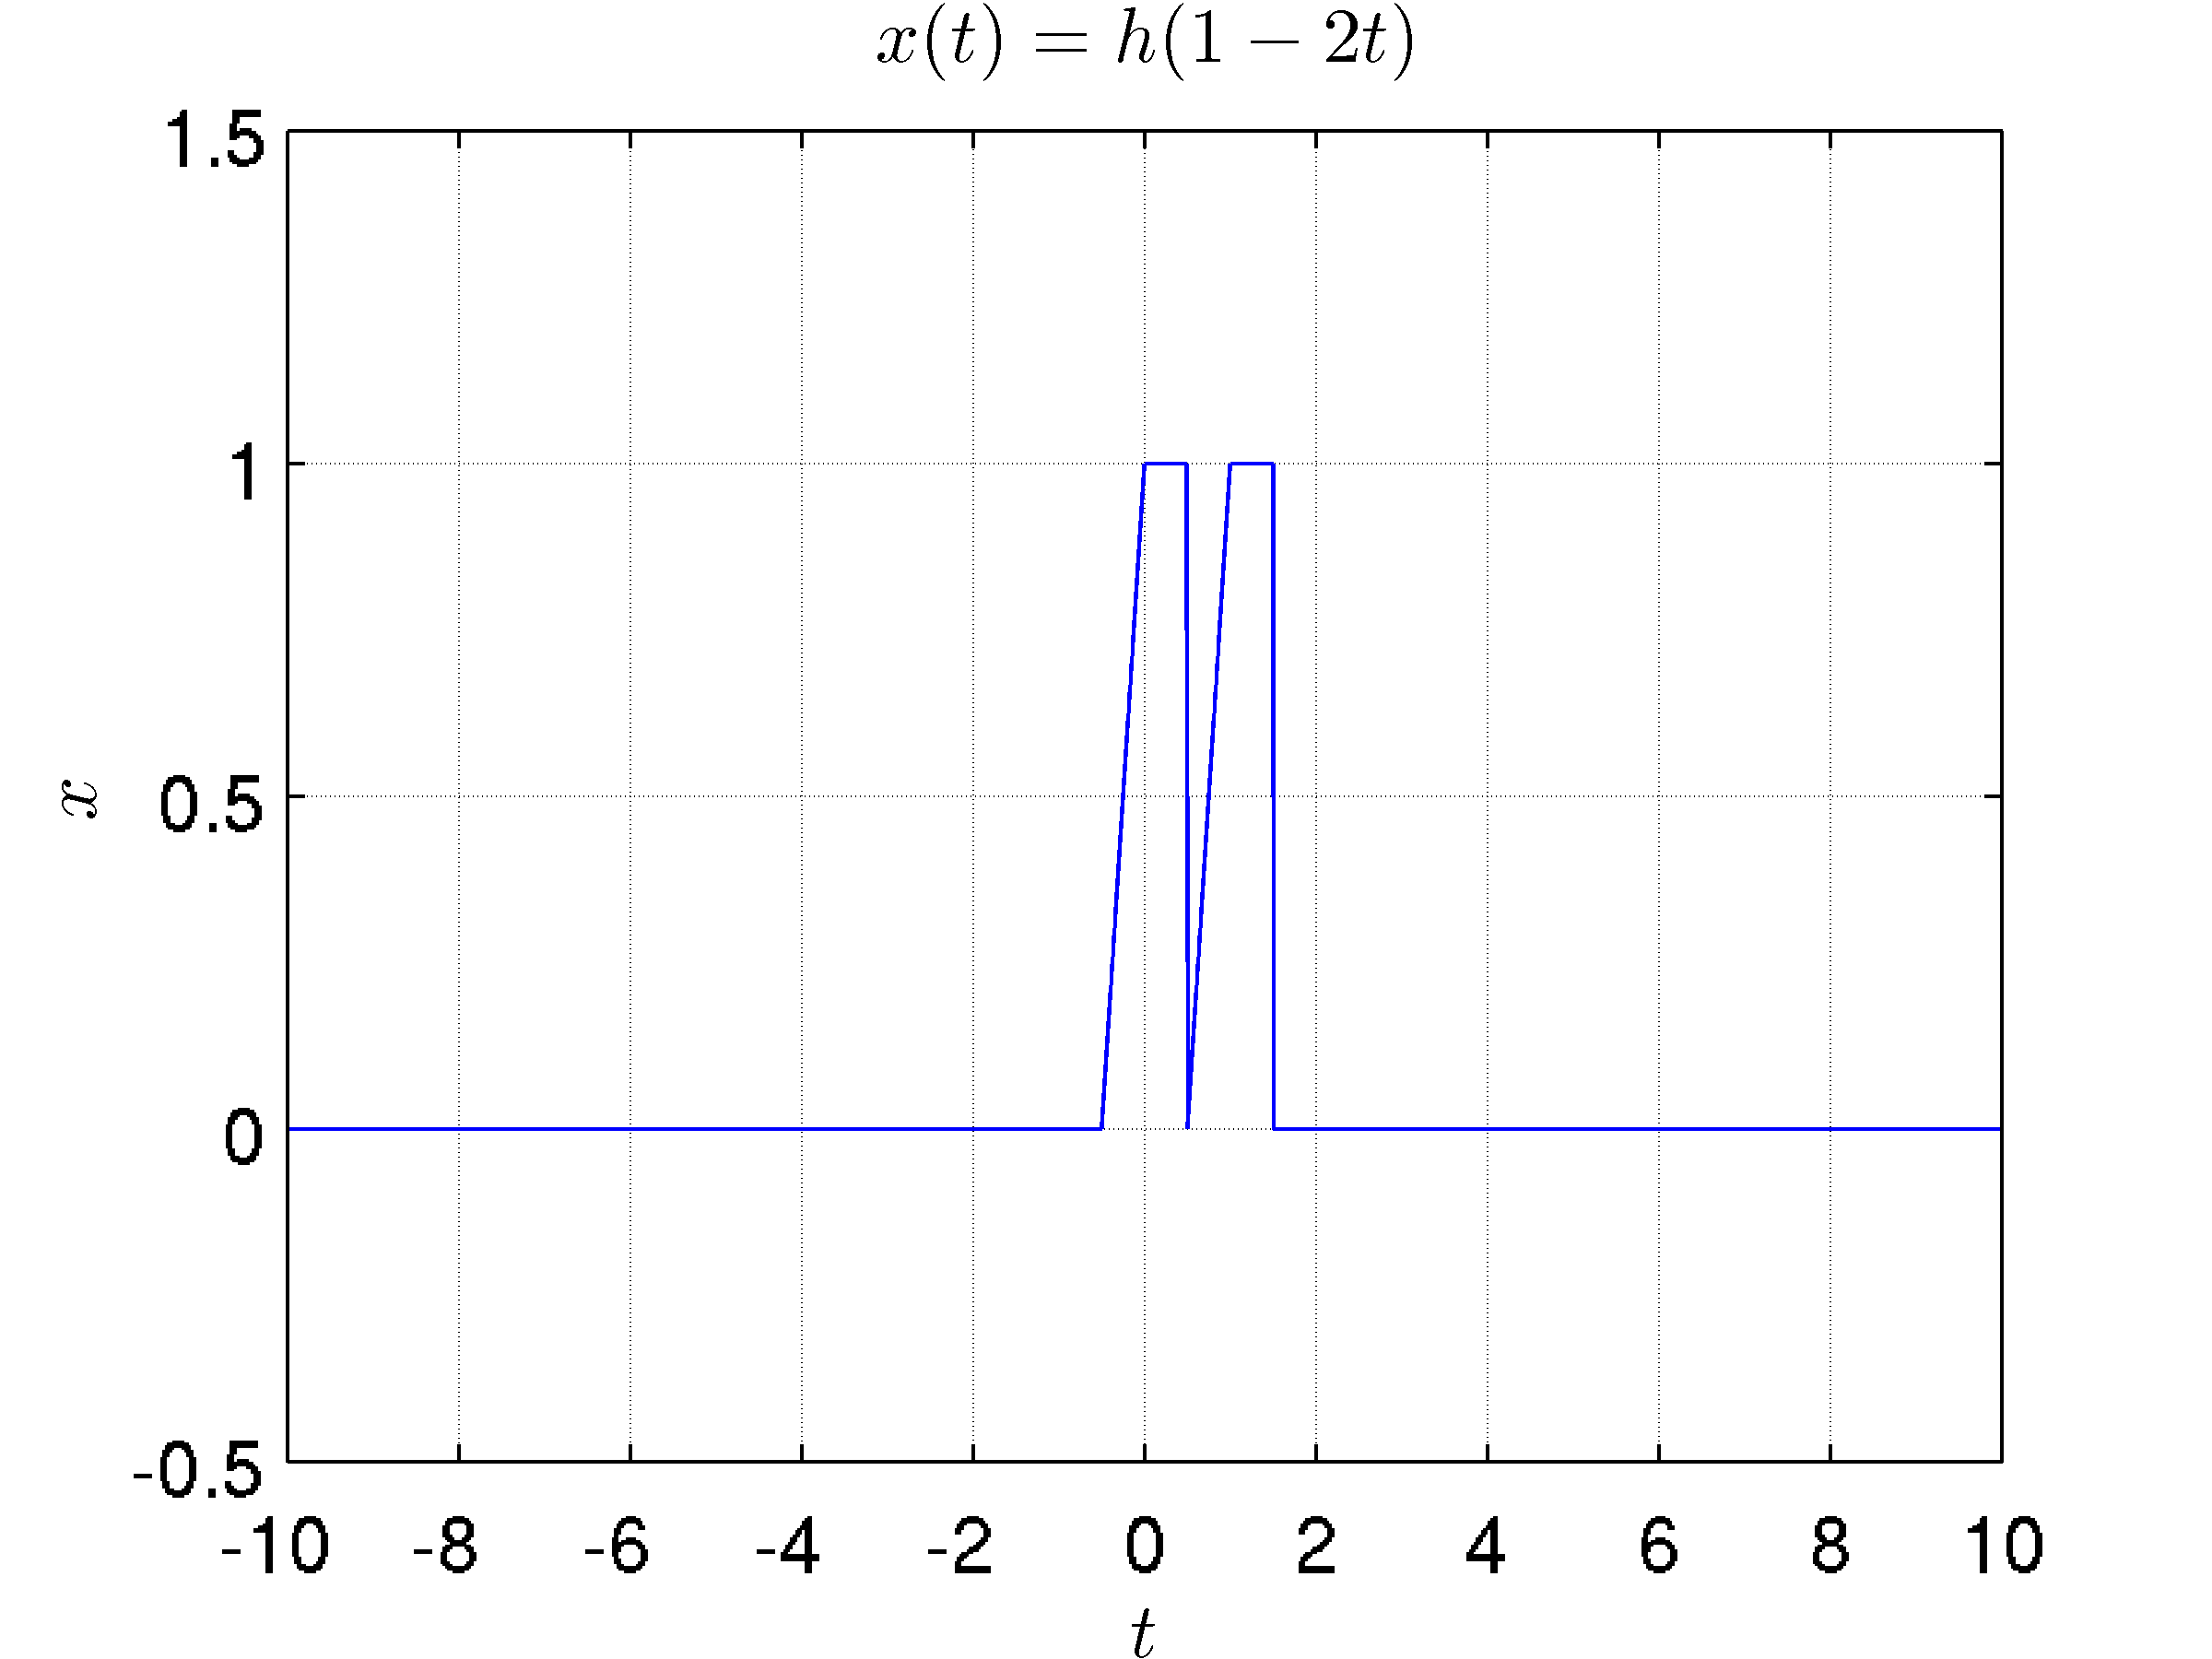
\includegraphics[width=3in]{./laboratorio_2/problema07_c.png}
        \vspace{0.7em}
        \vspace{0.1em}
        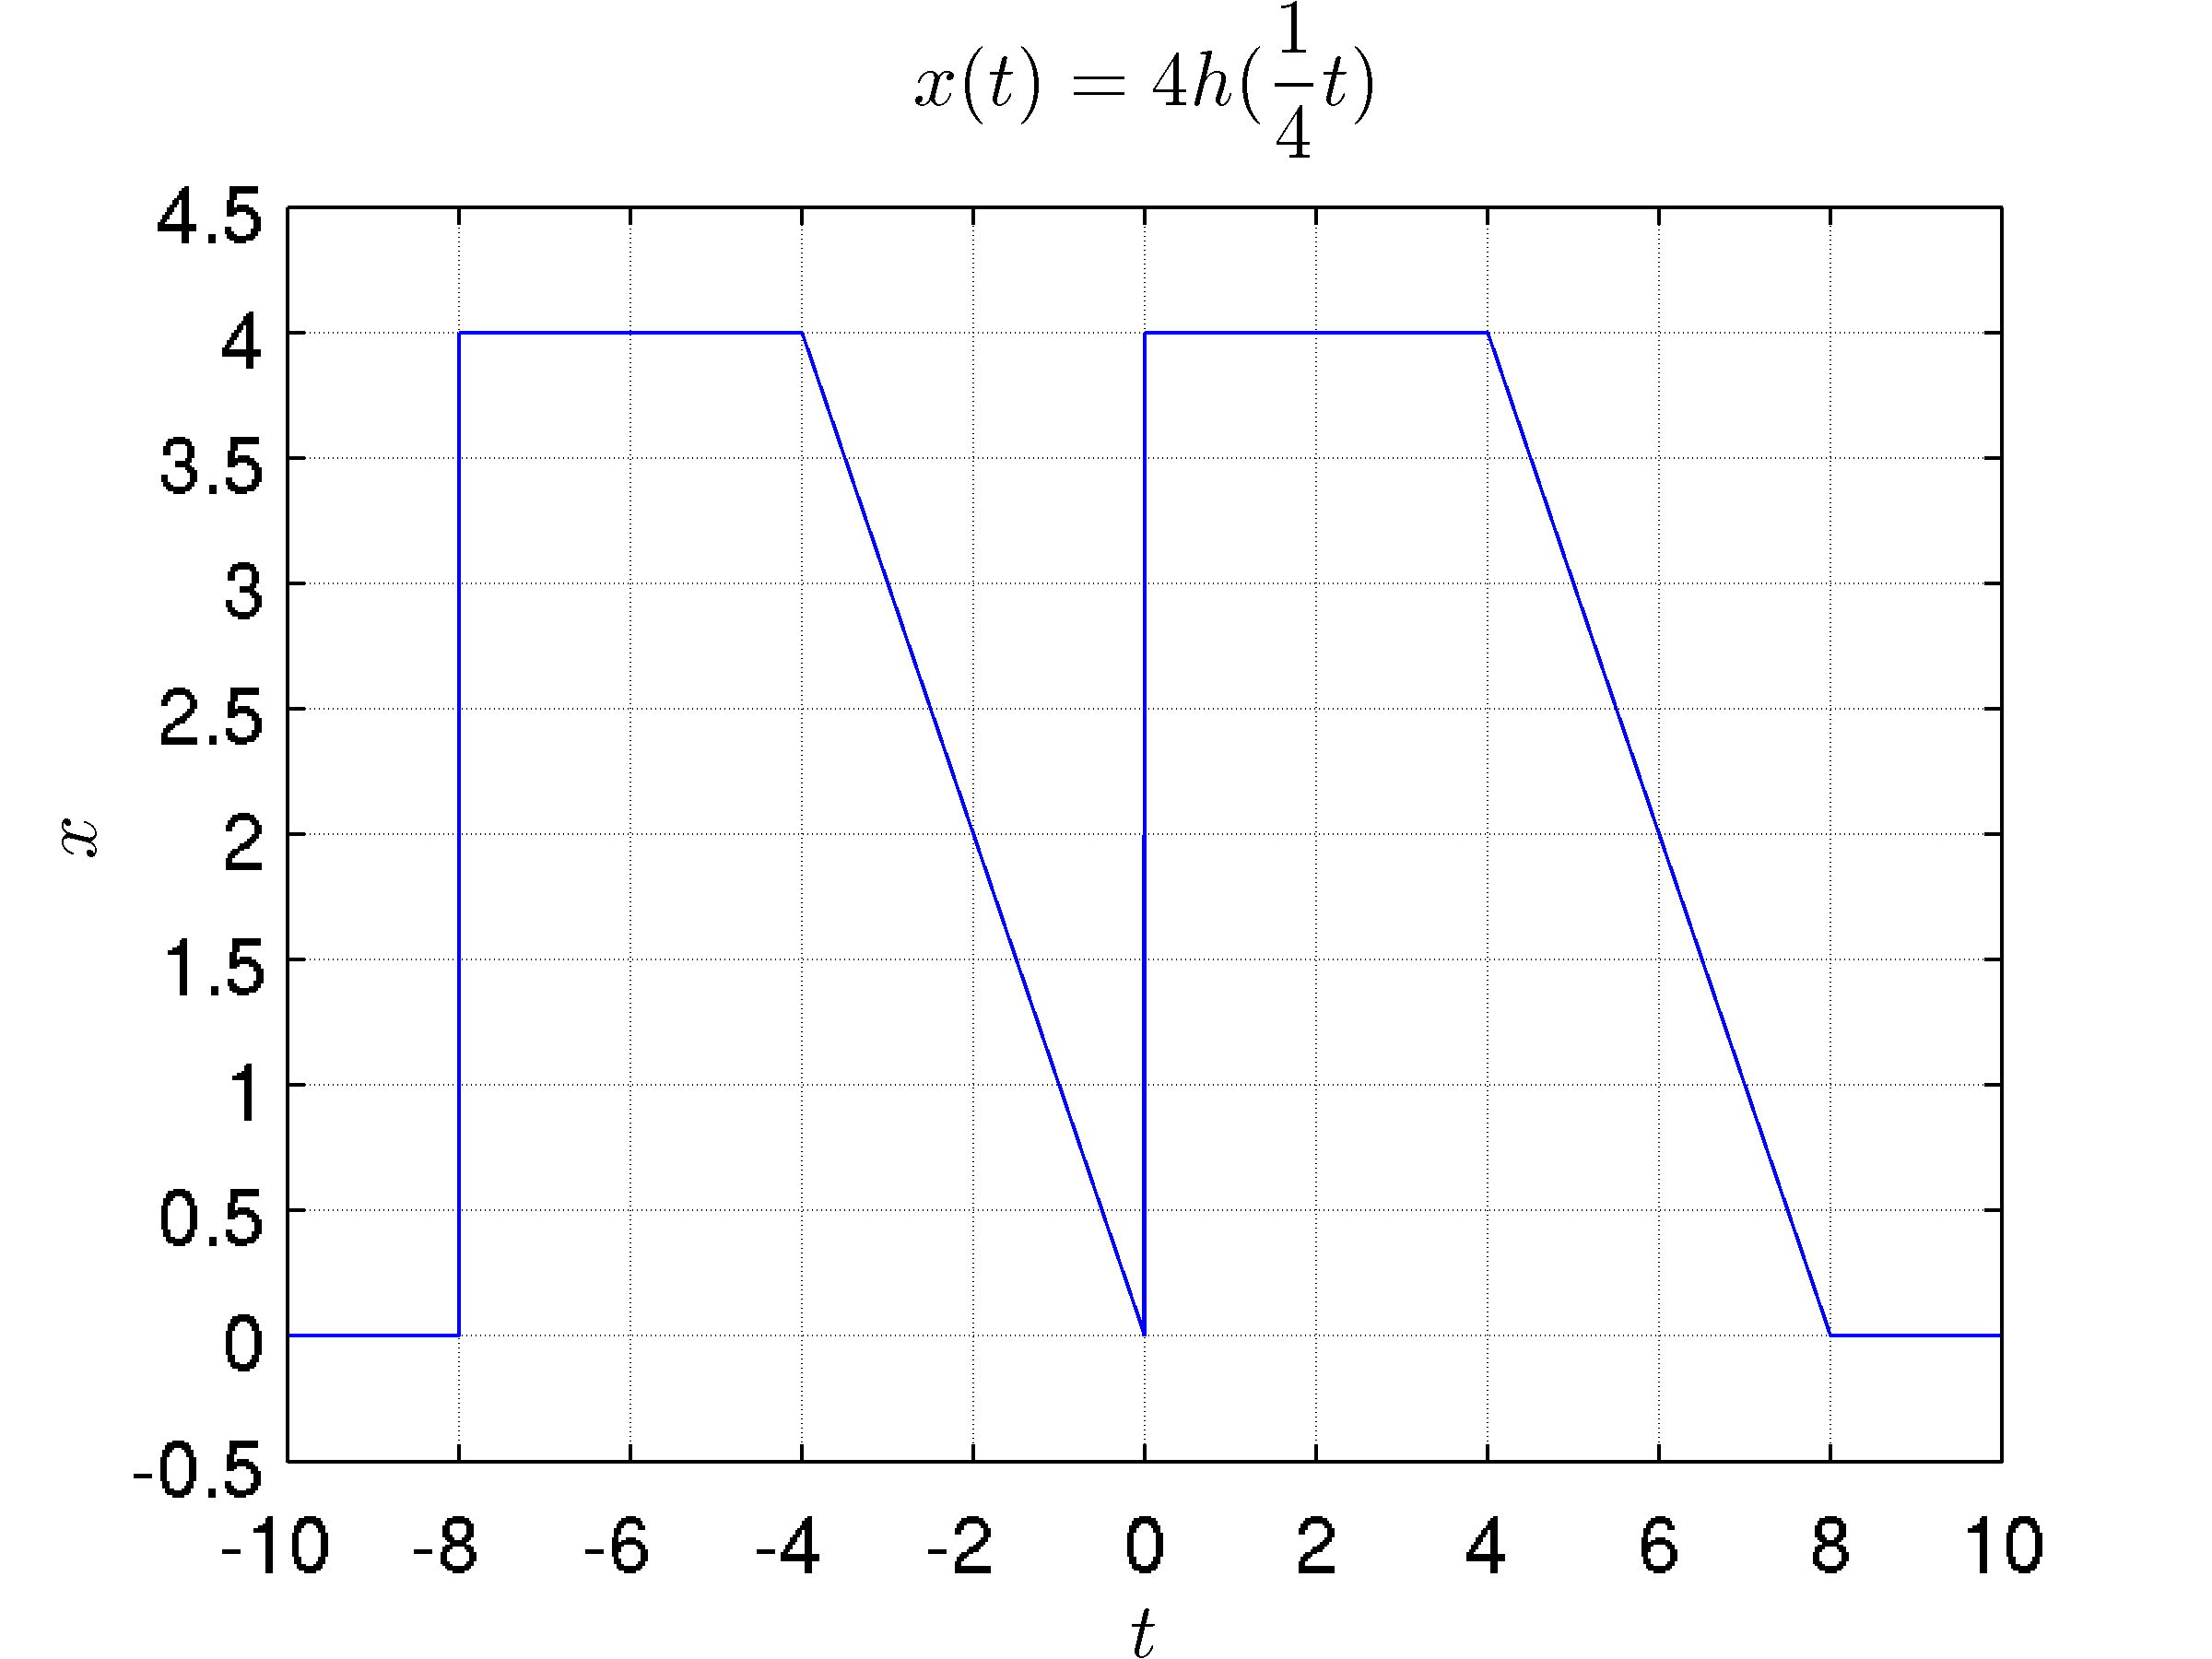
\includegraphics[width=3in]{./laboratorio_2/problema07_d.png}
        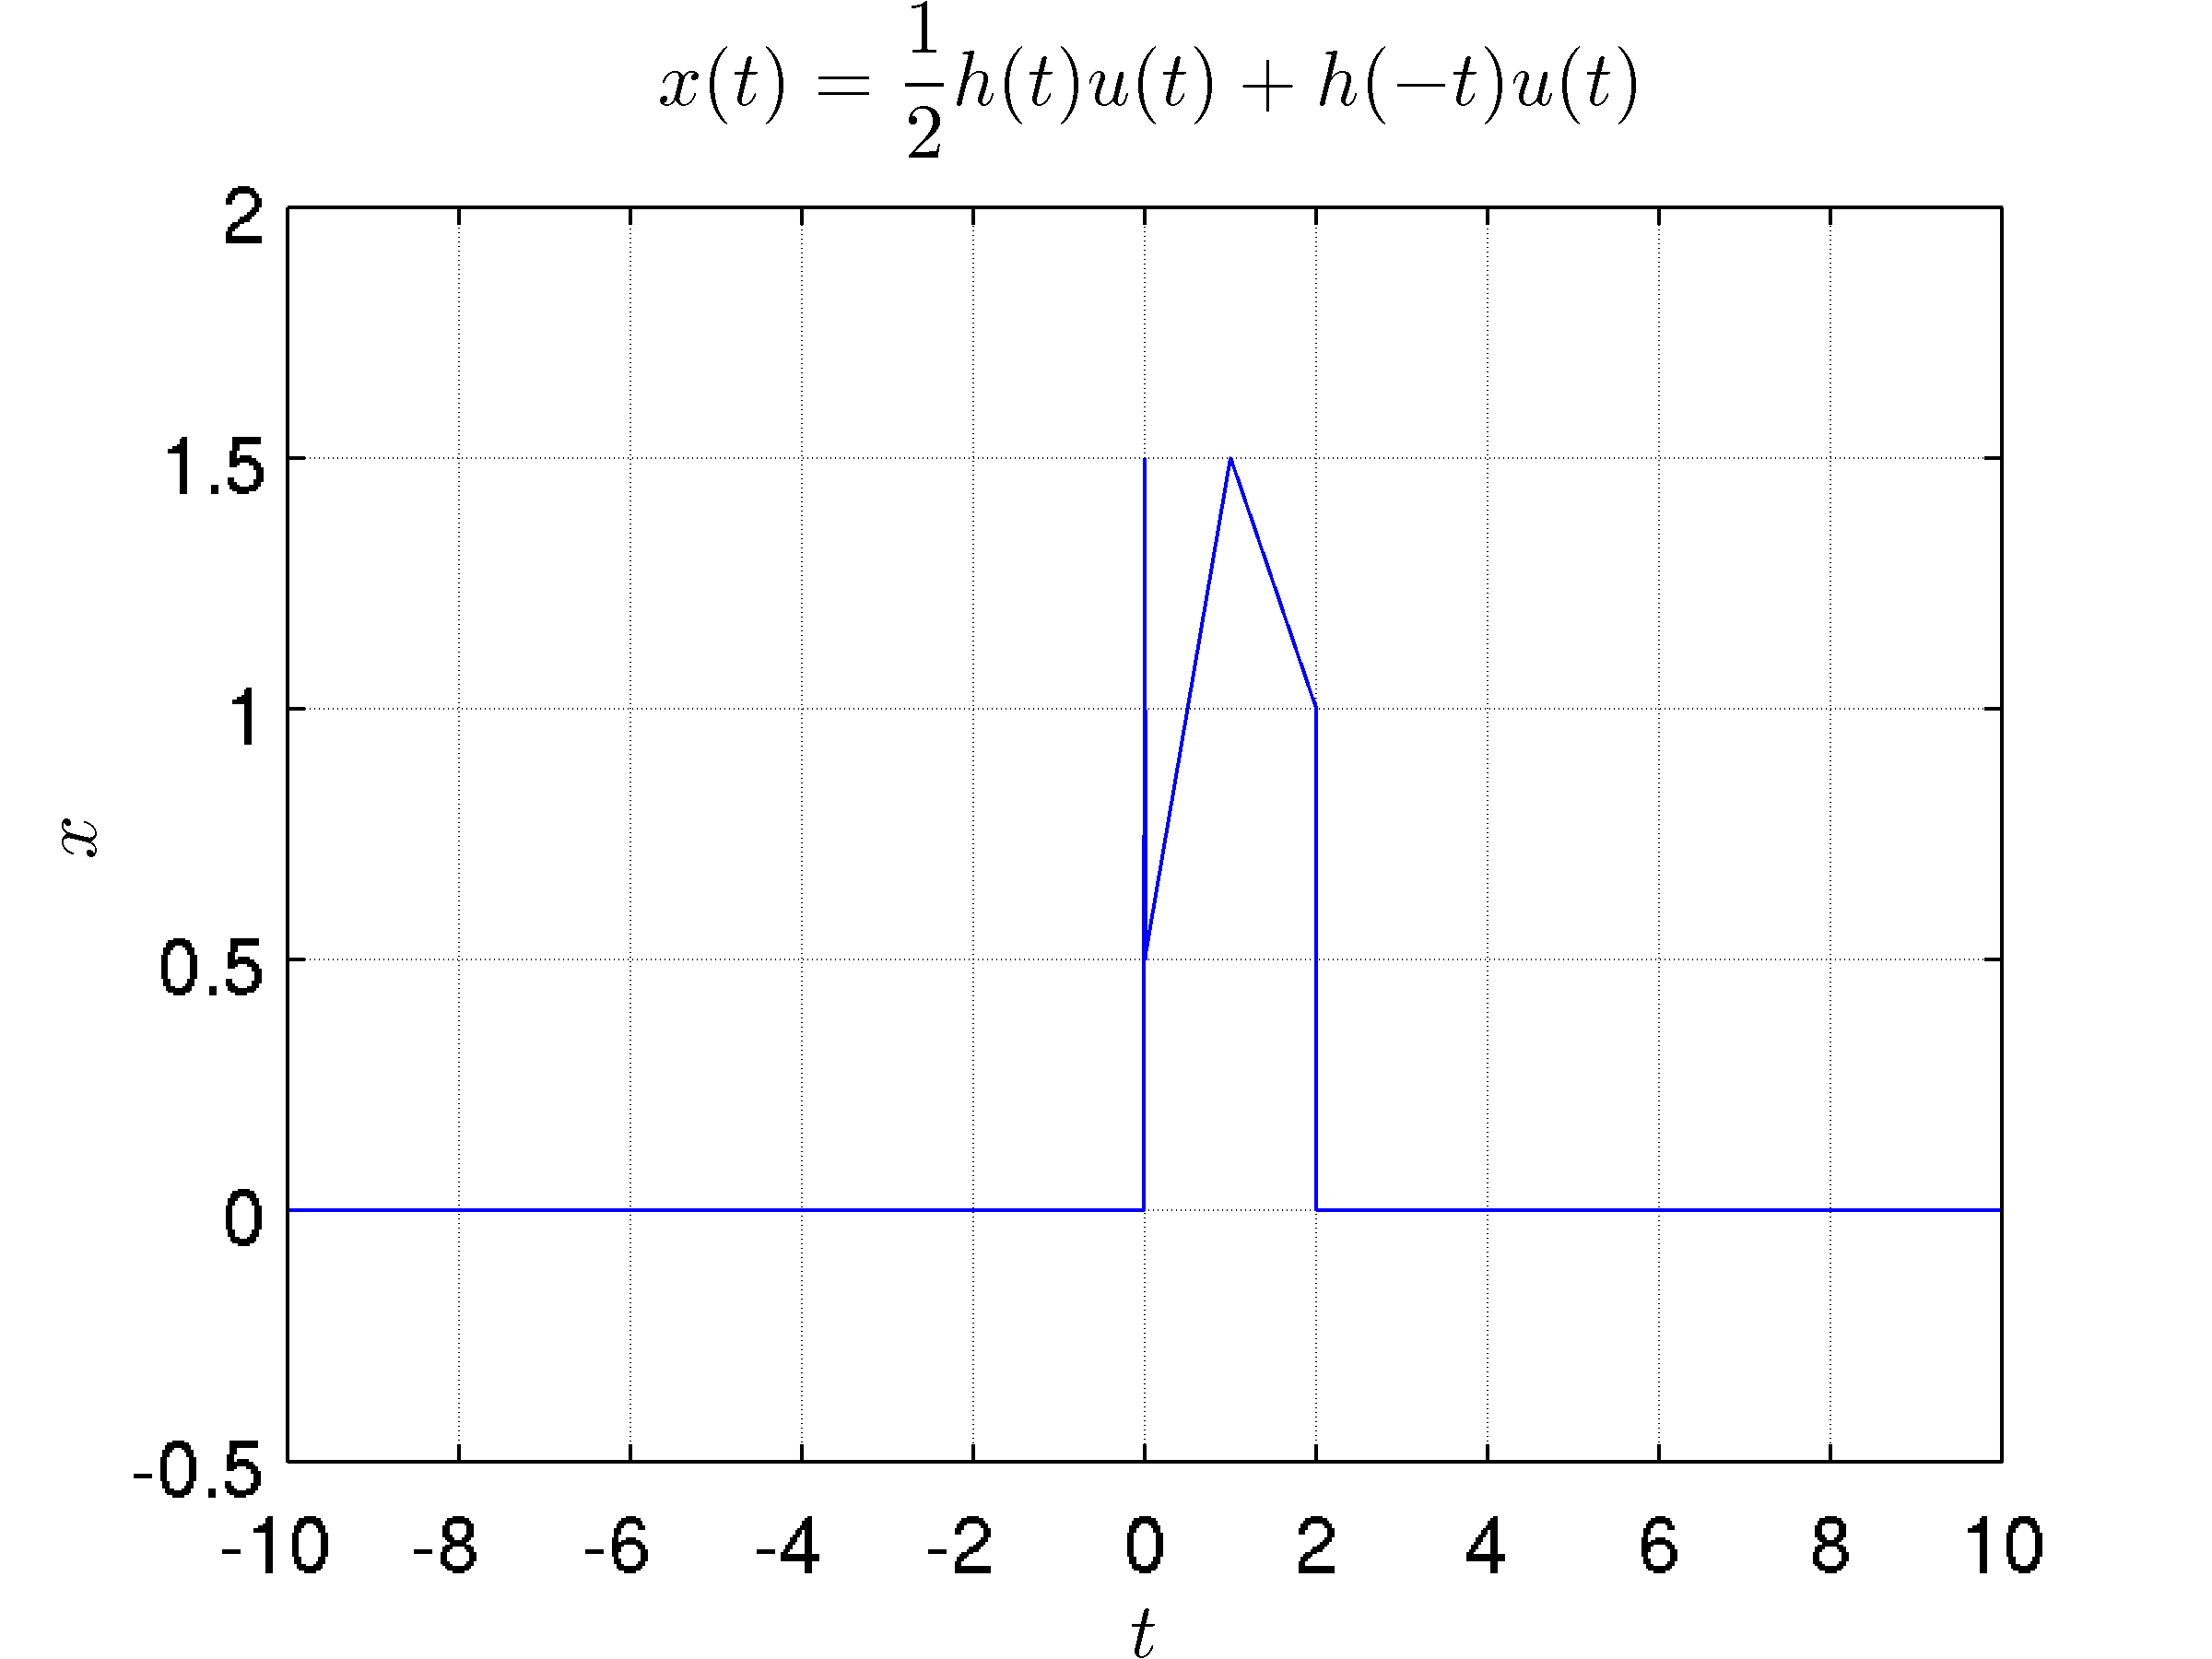
\includegraphics[width=3in]{./laboratorio_2/problema07_e.png}
        \vspace{0.7em}
        \vspace{0.1em}
        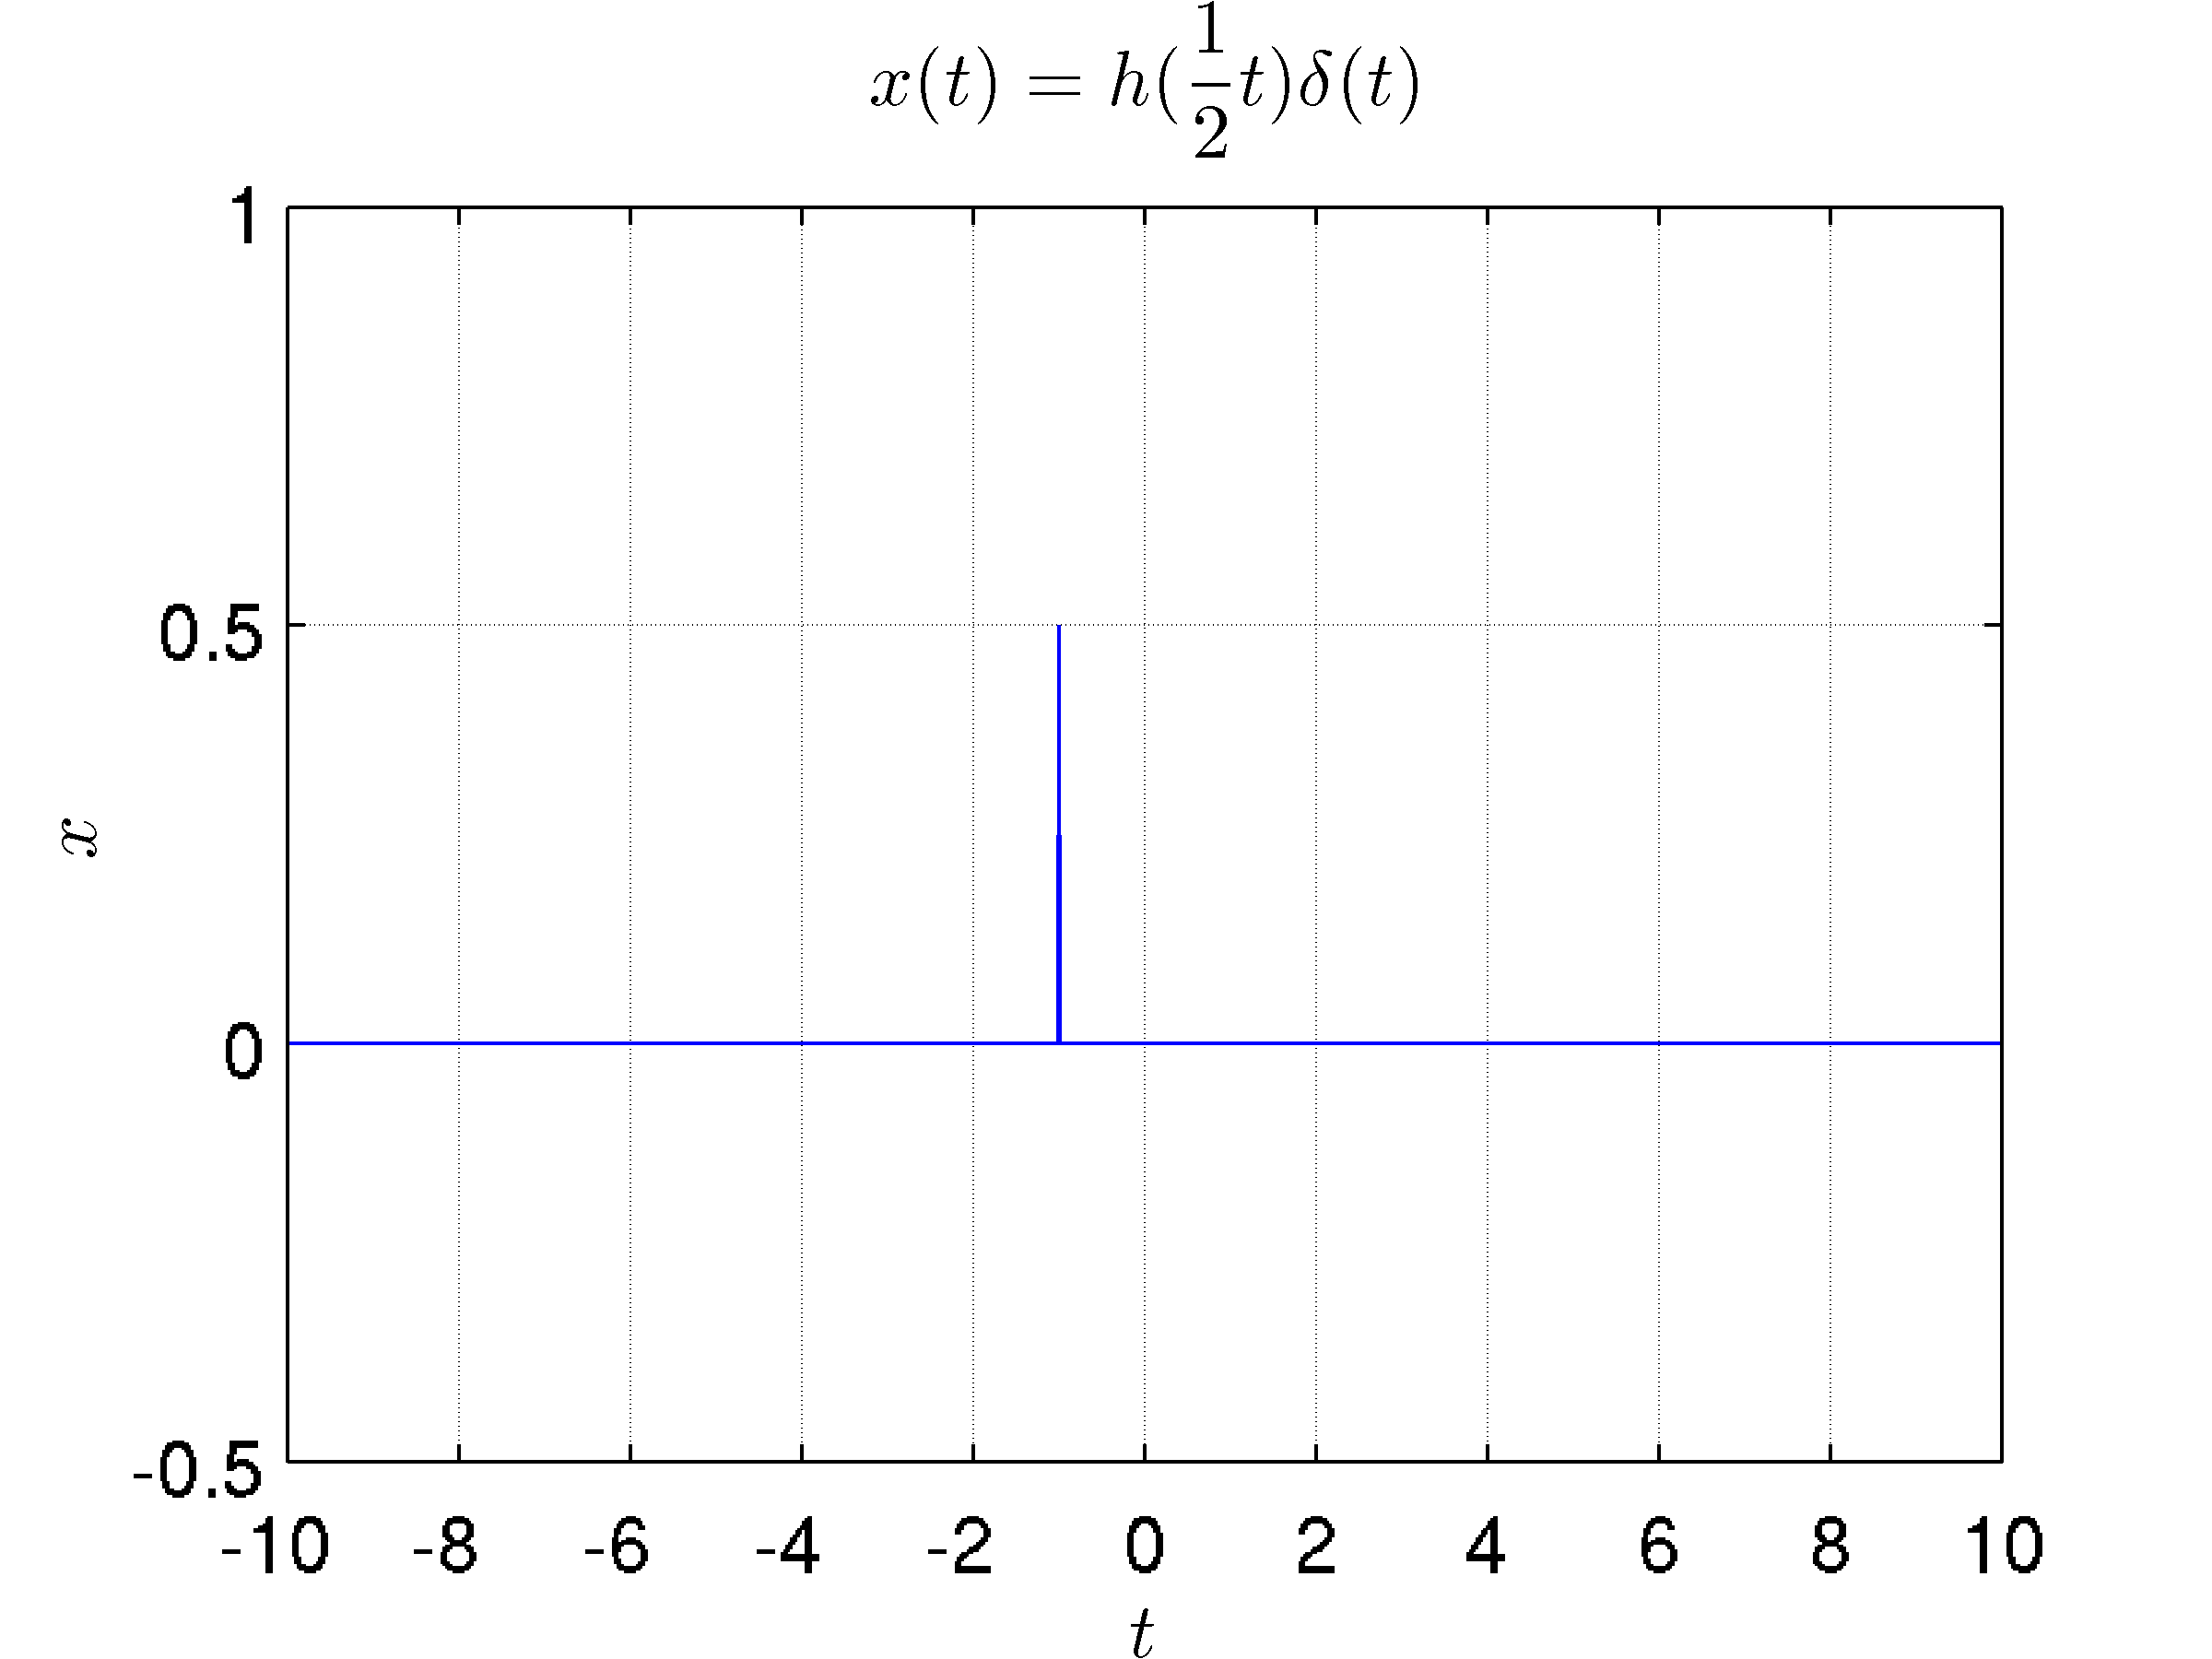
\includegraphics[width=3in]{./laboratorio_2/problema07_f.png}
        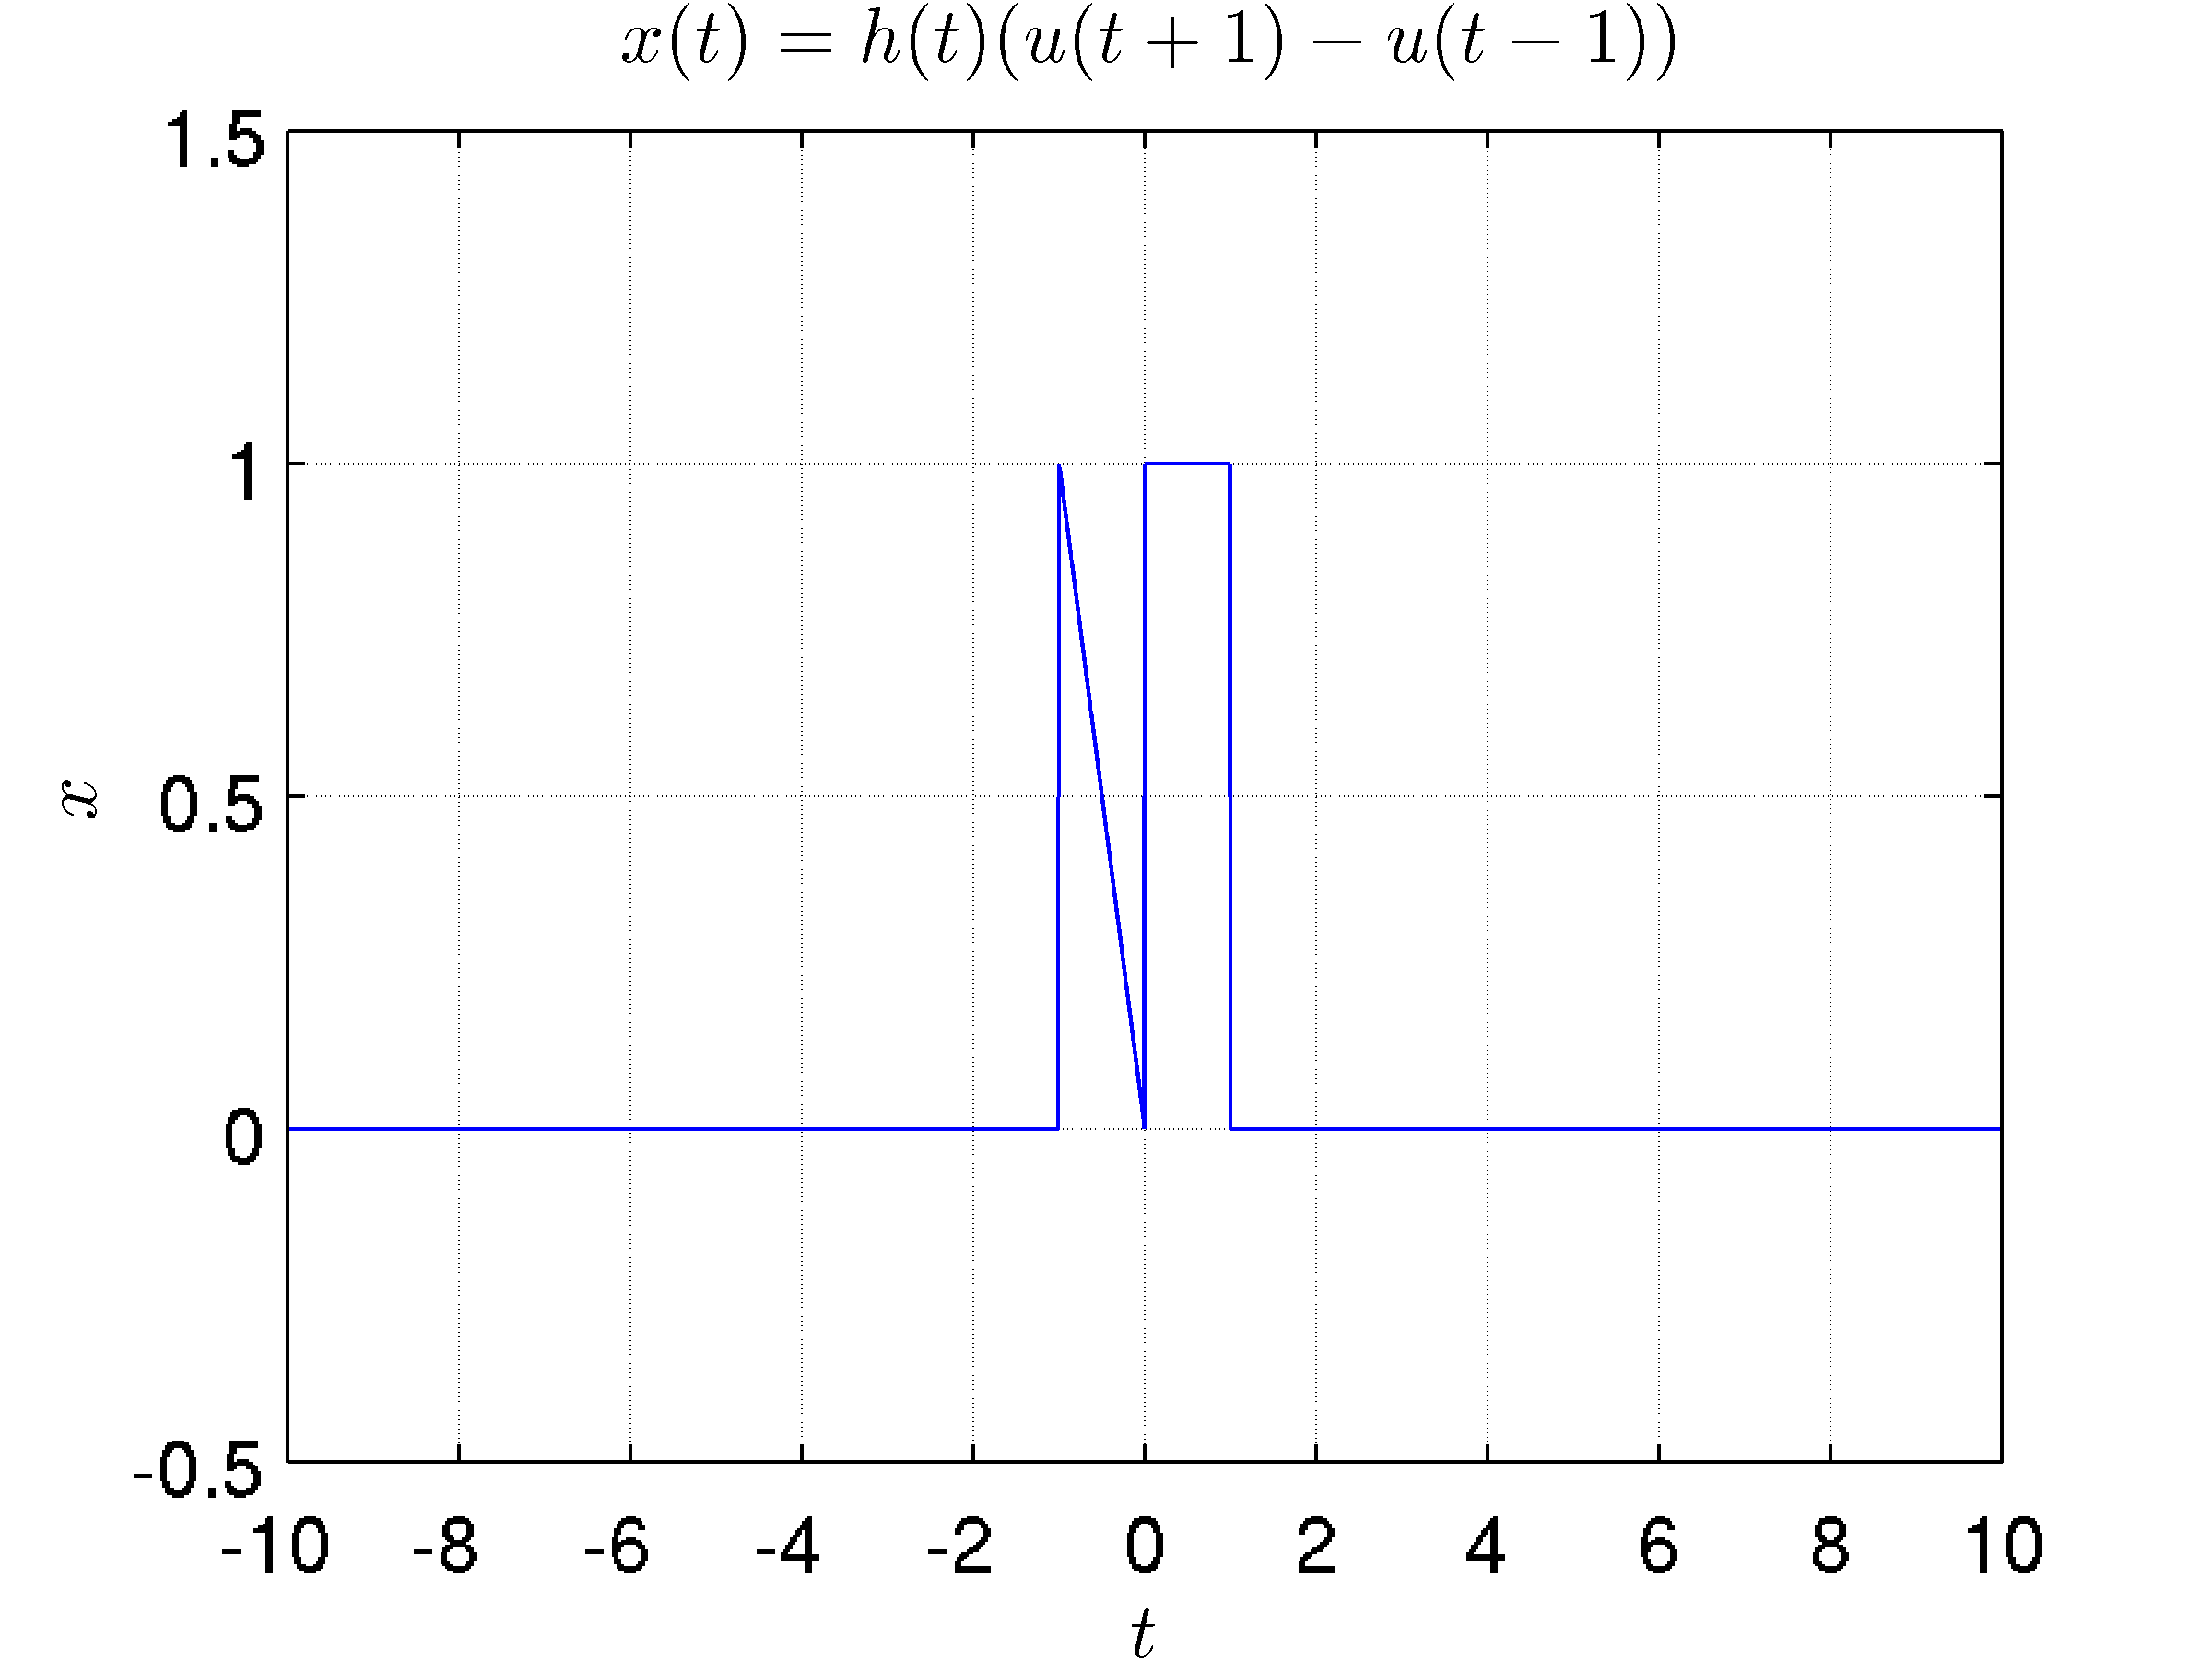
\includegraphics[width=3in]{./laboratorio_2/problema07_g.png}
      \end{figure}

\end{document}
